%%%%%%%%%%%%%%%%%%%%%%%%%%%%%%%%%%%%%%%%%%%%%%%%%%%%%%%%%%%%%%%%%%%%%%%%%%%%%%%%%%%%%%%%%%%%%%%%%%%%%%%%%%%%
\chapter[Analyse fréquentielle]{Analyse fréquentielle et représentation graphique\label{chap-anafreq}}
%%%%%%%%%%%%%%%%%%%%%%%%%%%%%%%%%%%%%%%%%%%%%%%%%%%%%%%%%%%%%%%%%%%%%%%%%%%%%%%%%%%%%%%%%%%%%%%%%%%%%%%%%%%%

%\section{Introduction}

Dans ce chapitre, nous allons établir la forme de la réponse d'un \SLCI~à une entrée sinuso\"idale, dite 
\textbf{réponse harmonique} en régime permanent.
Nous présenterons ensuite en détail les différentes représentations graphiques qui 
constitueront l'\textbf{analyse fréquentielle} de cette réponse harmonique.
Nous verrons en fin de chapitre une étude du transitoire dans des cas usuels.


%%%%%%%%%%%%%%%%%%%%%%%%%%%%%%%%%%%%%%%%%%%%%%%%%%%%%%%%%%%%%%%%%%%%%%%%%%%%%%%%%%%%%%%%%%%%%%%%%%%%%%%%%%%%
\section{Réponse harmonique}
%%%%%%%%%%%%%%%%%%%%%%%%%%%%%%%%%%%%%%%%%%%%%%%%%%%%%%%%%%%%%%%%%%%%%%%%%%%%%%%%%%%%%%%%%%%%%%%%%%%%%%%%%%%%

%L'excitation d'un \SLCI~par une entrée sinuso\"idale donne lieu, en régime permanent, 
%à une réponse harmonique dépendant de la fréquence d'excitation. 
%Nous allons ici établir la forme de cette réponse.

Soit un \SLCI~définit par une fonction de transfert $H(p)$ auquel on applique 
une entrée sinuso\"idale $e(t)$ tel que :
$$
e(t)=E_0\sin\omega t 
$$
d'amplitude $E_0$ et de pulsation $\omega$\footnote{Strictement, $\omega$ est une 
pulsation en unité \unit{}{\radian\per\second}, la fréquence associée étant $f=\omega/2\pi$, 
en \unit{}{\reciprocal\second} ou \unit{}{\hertz}. Cependant, 
par abus de langage, il est courant de se référer en terme de fréquence en parlant de la pulsation $\omega$. 
Nous prendrons cependant soin d'utiliser la bonne forme dans nos applications numériques.}.
Dans le domaine de Laplace, la sortie $S(p)$ est de la forme :
$$
S(p)=H(p)E(p)
$$
où $E(p)$ est la transformée de Laplace d'un sinus (c.f ligne 23 du tableau de l'\cref{annexe-lap}), 
on obtient alors :
$$
S(p)=H(p)\dfrac{E_0\omega}{p^2+\omega^2}
$$

Les pôles de la fonction de transfert $H(p)$ donnent lieu au 
régime transitoire alors que les pôles de l'excitation donnent 
lieu au régime permanent. 
Les deux pôles de l'excitation sont $p_{1,2}=\pm\jw$. La forme factorisée s'écrit alors:
$$
S(p)=H(p)\dfrac{E_0\omega}{(p+\jw)(p-\jw)}
$$

En régime permanent, la décomposition de $S(p)$ en éléments simples s'écrit :
$$
S(p)=\dfrac{A}{p-\jw} + \dfrac{B}{p+\jw}
$$

où les coéfficients s'obtiennent par évaluation :
\begin{align*}
    A&=(p-\jw)S(p)\bigg|_{p=\hphantom{-}\jw} =\dfrac{E_0\omega}{p+\jw}H(p)\bigg|_{p=\hphantom{-}\jw} =\hphantom{-}\dfrac{E_0}{2j}H(\jw)\\
    B&=(p+\jw)S(p)\bigg|_{p=-\jw}=\dfrac{E_0\omega}{p-\jw}H(p)\bigg|_{p=-\jw}=-\dfrac{E_0}{2j}H(-\jw)
\end{align*}

nous obtenons donc :
$$
S(p)=\dfrac{E_0}{2j}\left(\dfrac{H(\jw)}{p-\jw}-\dfrac{H(-\jw)}{p+\jw} \right)
$$

La transformée de Laplace inverse de la sortie $S(p)$ permet d'obtenir la réponse temporelle 
$$
s(t)=\dfrac{E_0}{2j}\left(H(\jw)e^{\jw t}-H(-\jw)e^{-\jw t}\right)
$$

En écrivant le nombre complexe $H(\jw)$ sous sa forme exponentielle (\Cref{annexe-NC}) :
\begin{align*}
    H(\jw)  &= |H(\jw)| e^{j\phi} \\
    H(-\jw) &= |H(\jw)| e^{-j\phi}
\end{align*}
où $|H(\jw)|$ et $\phi$ sont respectivement le module et l'argument du nombre complexe $H(\jw)$ 
et où l'on considère de plus que $H(-\jw)$ est égale à son conjugué (i.e $H(-\jw)=\overline{H(\jw)}$).

La réponse temporelle peut alors s'écrire sous la forme 
\begin{align*}
    s(t)=E_0|H(\jw)|\left(\dfrac{e^{j(\omega t+\phi)}-e^{-j(\omega t+\phi)}}{2j}\right)
\end{align*}
où l'on reconnait la forme exponentielle de la fonction sinus qui nous permet d'écrire :
\begin{bequation}[ams align]
    s(t)=E_0|H(\jw)|\sin{(\omega t+\phi)}\label{eq-rh}
\end{bequation}

Cette relation exprime que \textbf{l'excitation d'un {\protect{\SLCI}}~par une entrée sinuso\"idale donne 
lieu, en régime permanent, à une réponse harmonique dépendant de la fréquence d'excitation dont 
le gain en amplitude et la phase sont respectivement donné par le module et l'argument de la fonction
de transfert du système.}

\`A noter que $H(\jw)$ correspond au rapport de la sortie sur l'entrée,
ainsi le gain $|H(\jw)|$ et la phase peuvent être définits à partir de la sortie et de l'entrée du signal,
\begin{align*}
    H(\jw) &= \dfrac{S(\jw)}{E(\jw)} \\
    |H(\jw)|&= \dfrac{|S(\jw)|}{|E(\jw)|} \\
    \arg{H(\jw)}&=\arg{S(\jw)}-\arg{E(\jw)}
\end{align*}

Le gain $|H(\jw)|$ est une fonction réelle de $\omega$ de ce fait nous utiliserons par la suite
$G(\omega)$ pour noter plus explicitement cette dépendance. La phase est également
une fonction de la pulsation d'excitation, nous la noterons donc $\phi(\omega)$ par la suite.


%%%%%%%%%%%%%%%%%%%%%%%%%%%%%%%%%%%%%%%%%%%%%%%%%%%%%%%%%%%%%%%%%%%%%%%%%%%%%%%%%%%%%%%%%%%%%%%%%%%%%%%%%%%%
\subsection{Exemple de réponse harmonique dans le domaine temporelle}
%%%%%%%%%%%%%%%%%%%%%%%%%%%%%%%%%%%%%%%%%%%%%%%%%%%%%%%%%%%%%%%%%%%%%%%%%%%%%%%%%%%%%%%%%%%%%%%%%%%%%%%%%%%%
\index{Système du 1er ordre ! Réponse harmonique dans le domaine temporelle}
Considérons un \SLCI~définit par une fonction de transfert $H(p)$ du premier ordre (\Cref{eq-ft1er}) de forme canonique:
$$
H(p)=\dfrac{1}{1+p}
$$
avec $K=$1, $\tau=\unit{1}{\second}$.

Comme nous venons de le montrer la réponse harmonique est complétement 
déterminée par la connaissance du module et de l'argument du nombre complexe $H(\jw)$.
Le module donnant accès au rapport du gain en amplitude de la sortie sur l'entrée et 
l'argument à la différence de phase entre la sortie et l'entrée.

Calculons donc ces deux quantités pour notre fonction de transfert du premier ordre:
\begin{align*}
    G(\omega)   &=|H(\jw)|               =\left|\dfrac{1}{1+\jtw}\right|\\
    \phi(\omega)&=\arg\left(H(\jw)\right)=-\arctan(\omega\tau)
\end{align*}
Le~\cref{tab-1ertemp} présente le module et l'argument pour quelques valeurs particulières de $\omega$ 
($\omega=0.1$, $1$ et $\unit{10}{\rad\per\second}$).
\begin{table}
    \begin{center}
    \begin{tabular}{M{2.0cm}M{2.0cm}M{2.0cm}M{2.0cm}N}
        \hhline{====}
        $\omega \unit{}{[\rad\per\second]}$ & $\omega=1$    & $\omega=10$    & $\omega=100$ & \\[1.5em]
        \hline
        $G(\omega)$     & 0.99          & 0.70       & 0.1 & \\ [1.5em]
        \hline
   $\phi(\omega)$      &-5.7\degree  &-45\degree&-84.3\degree & \\[1.5em]
        \hhline{====}
    \end{tabular}
    \caption{Quelques valeurs particulières du gain et de la phase de la fonction de 
    transfert du premier ordre, pour $K=1$ et $\tau=\unit{1}{\second}$\label{tab-1ertemp}.}
    \end{center}
\end{table}
D'après ces valeurs, nous constatons que le rapport des amplitudes décroit et que le déphasage augmente 
lorsque la pulsation de l'excitation augmente.

La~\cref{fig-repham} présente la forme des réponses temporelles de ce système pour les données 
calculées du gain et de la phase de la fonction de transfert considérée. 
Cette représentation graphique montre ses limites, en effet quand est-il de toutes les autres valeurs de la pulsation ? 

Nous allons maintenant généraliser cette analyse sans pour autant avoir à 
tracer la réponse temporelle pour toutes les pulsations que l'on souhaite étudier.

\begin{figure}[!h]
\begin{center}
    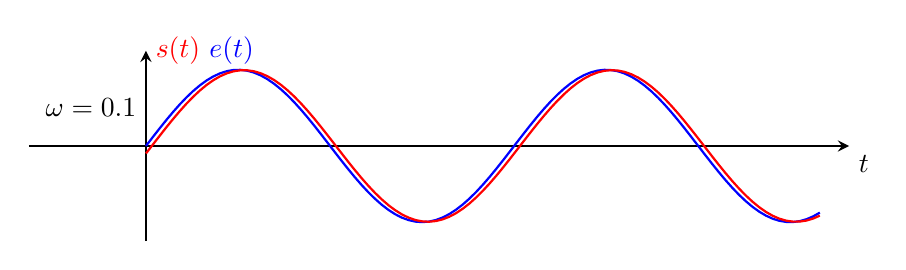
\begin{tikzpicture}
        \begin{axis}[
        ticks=none,
        axis line style = thick,
        height=4cm,
        width=12cm,
        axis x line=center,
        axis y line=center,
        xmin=-2,
        xmax=12,
        ymin=-1.25,
        ymax=1.25,
        xlabel={$t$},
        ylabel={\textcolor{red}{$s(t)$} \textcolor{blue}{$e(t)$}},
        xlabel style={below right},
        ylabel style={right},
        ]
            \addplot [thick,color=blue,domain=0:11.5, samples=101,unbounded coords=jump]{sin(deg(x))};
            \addplot [thick,color=red,domain=0:11.5, samples=101,unbounded coords=jump]{0.9950371902099892*sin(deg(x)-5.7)};
            \node[left] at (axis cs:0,0.5)  {$\omega=0.1$};
        \end{axis}
    \end{tikzpicture}
    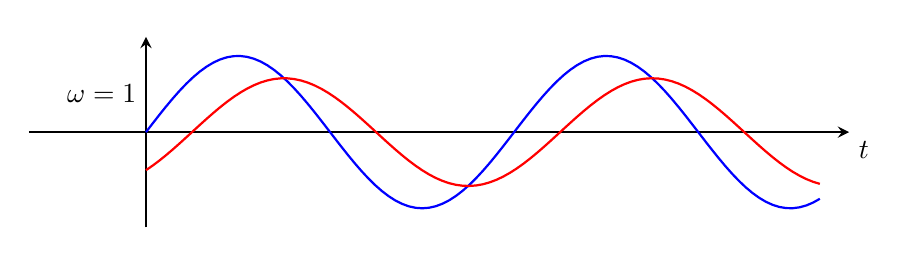
\begin{tikzpicture}
        \begin{axis}[
        ticks=none,
        axis line style = thick,
        height=4cm,
        width=12cm,
        axis x line=center,
        axis y line=center,
        xmin=-2,
        xmax=12,
        ymin=-1.25,
        ymax=1.25,
        xlabel={$t$},
        xlabel style={below right},
        ylabel={\hphantom{\textcolor{red}{$s(t)$} \textcolor{blue}{$e(t)$}}},
        ylabel style={right},
        ]
            \addplot [thick,color=blue,domain=0:11.5, samples=101,unbounded coords=jump]{sin(deg(x))};
            \addplot [thick,color=red,domain=0:11.5, samples=101,unbounded coords=jump]{0.707106*sin(deg(x)-45)};
            \node[left] at (axis cs:0,0.5)  {$\omega=1$};
        \end{axis}
    \end{tikzpicture}
    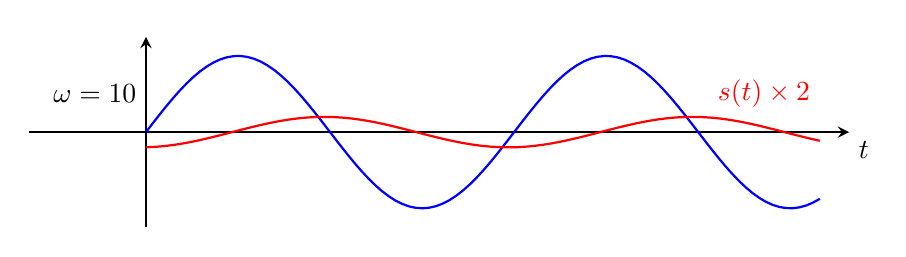
\begin{tikzpicture}
        \begin{axis}[
        ticks=none,
        axis line style = thick,
        height=4cm,
        width=12cm,
        axis x line=center,
        axis y line=center,
        xmin=-2,
        xmax=12,
        ymin=-1.25,
        ymax=1.25,
        xlabel={$t$},
        xlabel style={below right},
        ylabel={\hphantom{\textcolor{red}{$s(t)$} \textcolor{blue}{$e(t)$}}},
        ylabel style={right},
        ]
        \addplot [thick,color=blue,domain=0:11.5, samples=101,unbounded coords=jump]{sin(deg(x))};
        \addplot [thick,color=red,domain=0:11.5, samples=101,unbounded coords=jump]{0.2*sin(deg(x)-84.2894)};
        \node[left] at (axis cs:0,0.5)  {$\omega=10$};
            \node[left] at (axis cs:11.5,0.5)  {\textcolor{red}{$s(t)\times 2$}};
        \end{axis}
    \end{tikzpicture}
\caption{Réponse harmonique (en régime permanent) (\Cref{eq-rh}) d'un système du premier ordre
pour différentes pulsations d'excitation de la forme $e(t)=\sin{\omega t}$, (données du~\cref{tab-1ertemp}).
Cette figure permet d'observer l'augmentation du déphasage et la diminution 
de l'amplitude lorsque la fréquence d'excitations augmente. 
(bleu) excitation $e(t)$ (rouge) sortie $s(t)$.\label{fig-repham}}
\end{center}
\end{figure}

%>>> np.arctan(0.1)
%0.09966865249116204
%>>> np.arctan(1)
%0.7853981633974483
%>>> np.arctan(10)
%1.4711276743037347

%>>> np.arctan(0.1)*180/np.pi
%5.710593137499643
%>>> np.arctan(1)*180/np.pi
%45.0
%>>> np.arctan(10)*180/np.pi
%84.28940686250037
%>>> np.arctan(100)*180/np.pi
%89.42706130231653

%>>> abs(1./complex(1,0.1))
%0.9950371902099892
%>>> abs(1./complex(1,1))
%0.7071067811865476
%>>> abs(1./complex(1,10))
%0.09950371902099892




\newpage
%%%%%%%%%%%%%%%%%%%%%%%%%%%%%%%%%%%%%%%%%%%%%%%%%%%%%%%%%%%%%%%%%%%%%%%%%%%%%%%%%%%%%%%%%%%%%%%%%%%%%%%%%%%%
\section{Représentation graphique de la réponse harmonique}
%%%%%%%%%%%%%%%%%%%%%%%%%%%%%%%%%%%%%%%%%%%%%%%%%%%%%%%%%%%%%%%%%%%%%%%%%%%%%%%%%%%%%%%%%%%%%%%%%%%%%%%%%%%%

Comme nous venons de le voir, il est possible d'étudier
la réponse harmonique (en régime permanent) d'un \SLCI~dans le domaine 
temporel et observer la variation d'amplitude et du 
déphasage qui dépend de la pulsation d'excitation. Ces variations 
d'amplitude et de phase sont totalement déterminées par la 
connaissance du module et de l'argument du nombre complexe $H(\jw)$, c'est ce qui constitue 
l'analyse fréquentielle des \SLCI.

Dans cette partie, nous présenterons trois types de représentations graphiques, notamment :
\begin{itemize}
    \item le diagramme de Bode,
    \item le diagramme de Nyquist,
    \item et le diagramme de Black-Nichols. 
\end{itemize}
Nous étudierons en détail les diagrammes des 
modèles usuels que nous avons déjà rencontrés 
au chapitre précédent (\Cref{chap-model})

%Remarquons que la représentation 
Le terme \textbf{lieu de transfert} est communément utilisé pour parler du 
points de coordonnées $(\omega, \phi(\omega),G(\omega))$.



%%%%%%%%%%%%%%%%%%%%%%%%%%%%%%%%%%%%%%%%%%%%%%%%%%%%%%%%%%%%%%%%%%%%%%%%%%%%%%%%%%%%%%%%%%%%%%%%%%%%%%%%%%%%
\subsection{Diagramme de Bode}
%%%%%%%%%%%%%%%%%%%%%%%%%%%%%%%%%%%%%%%%%%%%%%%%%%%%%%%%%%%%%%%%%%%%%%%%%%%%%%%%%%%%%%%%%%%%%%%%%%%%%%%%%%%%
Un diagramme de Bode\footnote{Hendrik Wade Bode (1905-1982), ingénieur, chercheur 
et inventeur américain} permet de représenter le comportement fréquentielle 
d'un système quelconque en fonction de la fréquence d'excitation en entrée.
Il se compose de deux graphiques :
\begin{itemize}
    \item[i)] le tracé du gain en décibel en fonction de la pulsation $\omega$:
        \begin{bequation}[ams align] 
        G_{dB}(\omega)=20\log{G(\omega)}=20\log{|H(\jw)|} 
        \end{bequation}
    \item[ii)] le tracé de la phase en fonction de la pulsation $\omega$ :
        \begin{bequation}[ams align] 
        \phi(\omega)=\arg{H(\jw)}
        \end{bequation}
\end{itemize}
L'axe des pulsations étant généralement représenté par une échelle logarithmique 
pour permmettre la représentation de la réponse harmonique sur une large plage de valeurs en pulsation
(\Cref{annexe-log}). Le calcul de la phase passe lui par la détermination 
de l'argument principale (\Cref{annexe-NC}).

\begin{figure}[!h]
%\begin{center}
\centering
\begin{tikzpicture}
    \begin{axis}[
        name=axx,
        ticks=none,
        axis line style = thick,
        xmode=log,
        enlargelimits=false,
        height=4.cm,
        width=9cm,
        axis x line=center,
        axis y line=left,
        xmin=1e-2,
        xmax=1e2,
        ymin=-40,
        ymax=10,
        xlabel={$\log\omega$},
        xlabel style={below right},
        ylabel={$G_{dB}(\omega)$},
        ylabel style={left,rotate=-90,yshift=2.25em},
        clip=false,
        ]
        \addplot[ultra thick,color=black,domain=1e-2:1e2, samples=101,unbounded coords=jump]{-10*log10(1+x*x)};
        \draw[blue,dashed] (1e-2,{-10*log10(1+100)}) node[left] {$G_{dB}(\omega_2)$} -- (1e1,{-10*log10(1+100)}) ; 
        \draw[red ,dashed] (1e-2,{-10*log10(1+4)})   node[left] {$G_{dB}(\omega_1)$}   -- (2e0,{-10*log10(1+4)}) ; 
        \addplot [red, mark = *]  coordinates {(2e0,{-10*log10(1+4)})} {};
        \addplot [blue, mark = *] coordinates {(1e1,{-10*log10(1+100)})} {};
        \end{axis}
%\end{tikzpicture}
%\begin{tikzpicture}
        \begin{axis}[
        at={(axx.below south west)},yshift=-0.2cm,anchor=north west,
        ticks=none,
        axis line style = thick,
        xmode=log,
        enlargelimits=false,
        height=4.cm,
        width=9cm,
        axis x line=center,
        axis y line=left,
        xmin=1e-2,
        xmax=1e2,
        ymin=-90,
        ymax=20,
        xlabel={$\log\omega$},
        xlabel style={below right},
        ylabel={$\hphantom{_DB}\phi(\omega)$},
        ylabel style={left,rotate=-90,yshift=2.25em},
        clip=false,
        ]
        \addplot[ultra thick,color=black,domain=1e-2:1e2, samples=101,unbounded coords=jump]{-atan2(x,1)};
            \draw[blue,dashed] (1e1,{-atan2(1e1,1)})  -- node[left,yshift=0.5em] {$\omega_2$} (1e1,77) ; 
            \draw[red,dashed]  (2e0,{-atan2(2e0,1)})  -- node[left,yshift=-0.5em] {$\omega_1$} (2e0,100) ; 
        \draw[blue,dashed] (1e-2,{-atan2(1e1,1)}) node[left] {$\phi(\omega_2)$} -- (1e1,{-atan2(1e1,1)}) ; 
        \draw[red,dashed]  (1e-2,{-atan2(2e0,1)}) node[left] {$\phi(\omega_1)$} -- (2e0,{-atan2(2e0,1)}) ; 
        \addplot [red, mark = *]  coordinates {(2e0,{-atan2(2e0,1)})} {};
        \addplot [blue, mark = *] coordinates {(1e1,{-atan2(1e1,1)})} {};
        \end{axis}
\end{tikzpicture}
%\end{center}
\caption{Représentation schématique d'un diagramme de Bode. Le gain en décibel et la phase 
    associé à une fonction de transfert sont représentés en fonction de la pulsation (à l'échelle log) 
    sur deux repères distincts.}
\end{figure}

La principale propriété du diagramme de Bode est de permettre de simplifier un grand nombre calcul.
En effet, dans le cas par exemple où deux systèmes $H_1$ et $H_2$ sont mis en série,
$$                                                                                                                    
H(\jw)=H_1(\jw)H_2(\jw),
$$      
Le diagramme de Bode de $H(\jw)$ est la somme de deux diagrammes indépendants:
$$
\mathrm{Bode}(total)=\mathrm{Bode}(1)+\mathrm{Bode}(2)
$$
%$$
%les gains en décibels s'ajoutent :                                  
%$$                                                                                                                   
%G_{dB}(\omega)=20\log{|H_1(\jw)|} + 20\log{|H_2(\jw)|} = G_{dB1}(\omega) +  G_{dB2}(\omega) 
%$$                                                                                                                    
%de même pour la phase,                                                                                      
%$$                                                                                                                    
%\phi(\omega)=\arg{H_1(\jw)} + \arg{H_2(\jw)} = \phi_1(\omega) + \phi_2(\omega).
%$$                                                                                                                    
%\newpage
%%%%%%%%%%%%%%%%%%%%%%%%%%%%%%%%%%%%%%%%%%%%%%%%%%%%%%%%%%%%%%%%%%%%%%%%%%%%%%%%%%%%%%%%%%%%%%%%%%%%%%%%%%%%
\subsection{Diagramme de Nyquist}
%%%%%%%%%%%%%%%%%%%%%%%%%%%%%%%%%%%%%%%%%%%%%%%%%%%%%%%%%%%%%%%%%%%%%%%%%%%%%%%%%%%%%%%%%%%%%%%%%%%%%%%%%%%%

Un diagramme de Nyquist\footnote{Harry Nyquist (1889-1976), électronicien, ingénieur américain.} 
présente la partie imaginaire et la partie réelle de $H(\jw)$ pour différentes valeurs paramétrées de $\omega$.
Il a l'avantage de combiner les deux graphiques du diagramme 
de Bode en un seul. En effet, la phase et l'amplitude d'un point dans 
le plan complexe peut être déterminé graphiquement par respectivement l'angle 
avec l'axe des réels et la distance à l'origine (\Cref{annexe-NC}). 
Cette représentation graphique est communément appelée \textbf{le lieu de Nyquist}.
Le lieu de Nyquist complet est le tracé théorique des parties réel et imaginaire de $H(\jw)$, en considérant
les pulsations négatives, c'est à dire entre $\omega\rightarrow-\infty$ et $\omega\rightarrow+\infty$. 

\begin{figure}[!h]                                                                                                           
\begin{center}                                                                                                               
\begin{tikzpicture}
\begin{axis}
    [
    height=6.5cm,
    width=0.45\textwidth,
    axis lines = center,
    ticks=none,
    axis line style = thick,
    enlargelimits=false,
    xlabel=$\Re\left(H(\jw)\right)$,
    ylabel=$\Im\left(H(\jw)\right)$,
    xlabel style={below right},
    ylabel style={left},
    ymin=-10,
    ymax=+10,
    xmin=-10,
    xmax=+10
    ]     
    \def\xu{6.65043990901}
    \def\yu{3.24525022405}
    \def\xd{-2.6946926406}
    \def\yd{5.13601319826}
    \addplot [black, mark = *] coordinates {( 0, 0)} {};
    \node    [below]       at (axis cs:  7.853981633974483, 0)   {\scriptsize$\omega=0$};                
    \addplot [black, mark = *] coordinates {(7.853981633974483, 0)} {};                          
    \node    [below]       at (axis cs:  -2.2, 0) {\scriptsize$\omega\rightarrow\infty$};
    \addplot [red, mark = *] coordinates {(\xu,\yu)} {};
    \node    [above right, red]       at (axis cs:  \xu,\yu) {\scriptsize$\omega_1$};
    \draw    [red,thick] (axis cs:0,0) -- (axis cs: \xu,\yu)   node[midway,yshift=1.1em,xshift=0.6em] {\scriptsize$G(\omega_1)$};
    \draw    [red,thick] (axis cs:2.6,0) arc (0:18:1cm)      node[midway,yshift=0.23em,xshift=1.6em] {\scriptsize$\phi(\omega_1)$};
    \addplot [blue, mark = *] coordinates {( \xd,\yd)} {};
    \node    [above left, blue]       at (axis cs:  \xd,\yd) {\scriptsize$\omega_2$};
    \draw    [blue,thick] (axis cs:0,0) -- (axis cs:  \xd,\yd) node[midway,yshift=-0.5em,xshift=-1em] {\scriptsize$G(\omega_2)$};
    \draw    [blue,thick] (axis cs:1.9,0) arc (0:119:1.9)    node[midway,yshift=-1.7em,xshift=-1.85em] {\scriptsize$\phi(\omega_2)$};
    \addplot [postaction={decorate, decoration={markings,
              mark=at position 0.105 with {\arrow[rotate=-180]{latex};},
              mark=at position 0.31 with  {\arrow[rotate=-180]{latex};},
              mark=at position 0.51 with  {\arrow[rotate=-180]{latex};},
              mark=at position 0.71 with  {\arrow[rotate=-180]{latex};},
              mark=at position 0.9 with   {\arrow[rotate=-180]{latex};}
              }},thick,domain=0:7.853981633974483,samples=100]({x*sin(deg(x))},{x*cos(deg(x))});
\end{axis}
\end{tikzpicture}%
\hspace{0cm}
\begin{tikzpicture}
\begin{axis}
    [
    height=6.5cm,
    %width=8cm,
    width=0.45\textwidth,
    axis lines = center,
    ticks=none,
    axis line style = thick,
    enlargelimits=false,
    xlabel=$\Re\left(H(\jw)\right)$,
    ylabel=$\Im\left(H(\jw)\right)$,
    xlabel style={below right},
    ylabel style={left},
    ymin=-10,
    ymax=+10,
    xmin=-10,
    xmax=+10
    ]     
    \def\xu{6.65043990901}
    \def\yu{3.24525022405}
    \def\xd{-2.6946926406}
    \def\yd{5.13601319826}
 %   \addplot [black, mark = *] coordinates {( 0, 0)} {};
%    \node [below]       at (axis cs:  7.853981633974483, 0)   {$\omega=0$};                
 %   \addplot [black, mark = *] coordinates {(7.853981633974483, 0)} {};                          
%    \node [below right]       at (axis cs:  0, 0) {$\omega\rightarrow\infty$};
 %   \addplot [red, mark = *] coordinates {(\xu,\yu)} {};
 %   \node [above right, red]       at (axis cs:  \xu,\yu) {$\omega_1$};
%    \draw[red] (axis cs:0,0) -- (axis cs: \xu,\yu)   node[midway,yshift=1.4em,xshift=0.7em] {$G(\omega_1)$};
%    \draw[red] (axis cs:2.6,0) arc (0:22:1cm)      node[midway,yshift=0.23em,xshift=1.6em] {$\phi(\omega_1)$};
 %   \addplot [blue, mark = *] coordinates {( \xd,\yd)} {};
 %   \node [above left, blue]       at (axis cs:  \xd,\yd) {$\omega_2$};
%    \draw[blue] (axis cs:0,0) -- (axis cs:  \xd,\yd) node[midway,yshift=-0.8em,xshift=-1.5em] {$G(\omega_2)$};
%    \draw[blue] (axis cs:1.9,0) arc (0:119:1.9)    node[midway,yshift=-2em,xshift=-3.0em] {$\phi(\omega_2)$};
    \addplot [postaction={decorate, decoration={markings,
            mark=at position 0.105 with {\arrow[rotate=-180]{latex};},
            mark=at position 0.31 with  {\arrow[rotate=-180]{latex};},
            mark=at position 0.51 with  {\arrow[rotate=-180]{latex};},
            mark=at position 0.71 with  {\arrow[rotate=-180]{latex};},
            mark=at position 0.9 with   {\arrow[rotate=-180]{latex};}
             }},thick,domain=0:7.853981633974483,samples=100]({x*sin(deg(x))},{x*cos(deg(x))});
    \addplot [postaction={decorate, decoration={markings,
            mark=at position 0.105 with {\arrow{latex};},
            mark=at position 0.31 with  {\arrow{latex};},
            mark=at position 0.51 with  {\arrow{latex};},
            mark=at position 0.71 with  {\arrow{latex};},
            mark=at position 0.9 with   {\arrow{latex};}
      }},dashed,thick,domain=0:7.853981633974483,samples=100]({x*sin(deg(x))},{-x*cos(deg(x))});
\end{axis}
\end{tikzpicture}
\end{center}
    \caption{ (gauche) Représentation schématique d'un diagramme de Nyquist. Le nombre complexe 
    $H(\jw)$ est représenté dans le plan complexe pour différentes valeurs de la 
    pulsation $\omega$ de 0 à $\infty$. (droite) Représentation schématique du lieu complet de Nyquist, 
    symmétrique par rapport à l'axe des réels.\label{fig-nyquist}}
\end{figure}


%%%%%%%%%%%%%%%%%%%%%%%%%%%%%%%%%%%%%%%%%%%%%%%%%%%%%%%%%%%%%%%%%%%%%%%%%%%%%%%%%%%%%%%%%%%%%%%%%%%%%%%%%%%%
\subsection{Diagramme de Black}
%%%%%%%%%%%%%%%%%%%%%%%%%%%%%%%%%%%%%%%%%%%%%%%%%%%%%%%%%%%%%%%%%%%%%%%%%%%%%%%%%%%%%%%%%%%%%%%%%%%%%%%%%%%%
Le diagramme de Black\footnote{Il également appelé diagramme de Nichols ou encore Black-Nichols.} 
consiste à tracer le gain en décibel $G_{dB}(\omega)$ 
en fonction de la phase, paramétré par la pulsation $\omega$. À l'instar du diagramme de Nyquist, le diagramme 
de Black à l'avantage de combiner les deux graphiques du diagramme de Bode.
La diagramme de Black est habituellement utilisé dans l'étude des systèmes asservis (\Cref{chap-asservis}) 
pour déterminer le lieu de transfert dans le plan de Black d'un système en boucle fermée (FTBF) à partir 
de la connaissance du lieu de transfert dans le plan de Black de la Fonction de Transfert en Boucle ouverte (FTBO).

%(moins important dans une premiere découverte des \SLCI.
%Il pourra être introduit séparemment dans le cas des systèmes asservis.)

\begin{figure}[!h]                                                                                                           
\begin{center}                                                                                                               
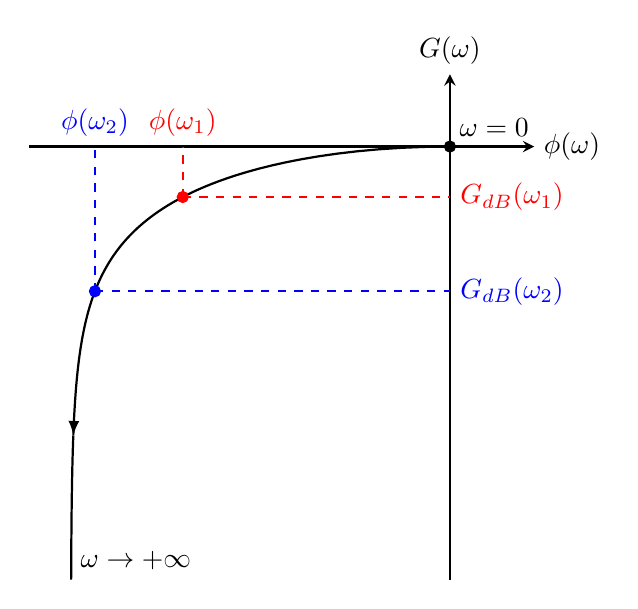
\begin{tikzpicture}
\begin{axis}
    [
    clip=false,
    height=8cm,
    width=8cm,
    ticks=none,
    axis lines = center,
    axis line style = thick,
    enlargelimits=false,
    ylabel=$G(\omega)$,
    xlabel=$\phi(\omega)$,
    xlabel style={right},
    ylabel style={above},
    xticklabel style={above,yshift=0.3em},
    yticklabel style={right,xshift=0.3em},
    ymin=-60,
    ymax=+10,
    xmin=-100,
    xmax=+20
    ]     
    \addplot [thick,domain=0:10,samples=100] ({-atan2(x,1)},{-10*log10(1+x*x)});
    \addplot [thick,domain=10:100,samples=100,-latex] ({-atan2(x,1)},{-10*log10(1+x*x)});
    \addplot [thick,domain=100:1000,samples=100] ({-atan2(x,1)},{-10*log10(1+x*x)});
    \addplot [black, mark = *] coordinates {( 0, 0)} {};                    
    \addplot [black, mark = *,blue] coordinates {({-atan2(10,1)},{-10*log10(1+10*10)} )} {};                    
    \draw[thick,blue,dashed] (axis cs: {-atan2(10,1)},{-10*log10(1+10*10)}) -- 
                            (axis cs: {-atan2(10,1)},0)  
                            node[above] {$\phi(\omega_2)$};
    \draw[thick,blue,dashed] (axis cs: {-atan2(10,1)},{-10*log10(1+10*10)}) -- 
                            (axis cs: 0,{-10*log10(1+10*10)}) 
                            node[right] {$G_{dB}(\omega_2)$} ;
    \addplot [black, mark = *,red] coordinates {({-atan2(2,1)},{-10*log10(1+4)} )} {};                    
    \draw[thick,red,dashed] (axis cs: {-atan2(2,1)},{-10*log10(5)}) -- 
                             (axis cs: {-atan2(2,1)},0) 
                            node[above] {$\phi(\omega_1)$};
    \draw[thick,red,dashed] (axis cs: {-atan2(2,1)},{-10*log10(5)}) -- 
                             (axis cs: 0,{-10*log10(5)}) 
                            node[right] {$G_{dB}(\omega_1)$} ;
    \node [above right]  at (axis cs: 0 , 0)   {$\omega=0$}; 
    \node [above right]  at (axis cs:-90, -60) {$\omega\rightarrow+\infty$}; 

\end{axis}
\end{tikzpicture}
\end{center}
\caption{Représentation schématique d'un diagramme de Black. Le gain et la phase 
    de la fonction de transfert $H(\jw)$ sont représentés sur le lieu de Black 
    pour différentes valeurs de la pulsation $\omega$ de 0 à $\infty$.\label{fig-black}}
\end{figure}


\newpage
%%%%%%%%%%%%%%%%%%%%%%%%%%%%%%%%%%%%%%%%%%%%%%%%%%%%%%%%%%%%%%%%%%%%%%%%%%%%%%%%%%%%%%%%%%%%%%%%%%%%%%%%%%%%
\section{Analyse fréquentielle des modèles usuels}
%%%%%%%%%%%%%%%%%%%%%%%%%%%%%%%%%%%%%%%%%%%%%%%%%%%%%%%%%%%%%%%%%%%%%%%%%%%%%%%%%%%%%%%%%%%%%%%%%%%%%%%%%%%%

Nous allons ici présenter la forme canonique des diagrammes fréquentielles (Bode, Nyquist et Black-Nichols) pour 
les modèles usuels rencontrées dans l'étude des \SLCI. Les diagrammes de Bode restent l'outil principale et fera 
l'objet d'une présentation plus détaillée.

\subsection{Diagrammes de Bode : méthodologie générale}
Pour chacuns des modèles usuels, nous appliquerons la procédure suivante :
\begin{itemize}
    \item Définir la fonction de transfert $H(p)$ du modèle pour $p=\jw$
    \item \'Etablir la fonction du gain $G(\omega)$ à partir du module de $|H(\jw)|$
    \item \'Etablir la fonction de la phase $\phi(\omega)$ à partir de l'argument principale de $|H(\jw)|$.
          L'argument principale est définit à l'\Cref{annexe-NC}.
    \item Si les fonctions $G(\omega)$ et $\phi(\omega)$ ne sont pas de simples constantes, réalisér une étude
        asymptotique pour $\omega\rightarrow 0$ et $\omega\rightarrow +\infty$.
    \item Tracer le diagramme de Bode \textbf{réel} et le diagramme de Bode \textbf{asymptotique}.
\end{itemize}

\newpage
%%%%%%%%%%%%%%%%%%%%%%%%%%%%%%%%%%%%%%%%%%%%%%%%%%%%%%%%%%%%%%%%%%%%%%%%%%%%%%%%%%%%%%%%%%%%%%%%%%%%%%%%%%%%
\subsubsection{Diagramme de Bode d'un gain pur}
%%%%%%%%%%%%%%%%%%%%%%%%%%%%%%%%%%%%%%%%%%%%%%%%%%%%%%%%%%%%%%%%%%%%%%%%%%%%%%%%%%%%%%%%%%%%%%%%%%%%%%%%%%%%
La fonction de transfert d'un gain pur est de la forme $H(\jw)=K$,
le gain est donc simplement donné par 
$$
G(\omega)=|H(\jw)|=K
$$ 
d'où le gain $G_{dB}$ en décibel :
\begin{bequation}[ams align*]
G_{dB}(\omega)= 20\log{K}
\end{bequation} ce qui correspond à une constante en gain (\Cref{fig-bode_gain}) 
et la phase s'obtient à partir de l'argument principale du nombre complexe $H(\jw)$:
\begin{bequation}[ams align*]
\phi(\omega) = 0
\end{bequation}

\begin{figure}[!htb]
\centering
\begin{tikzpicture}[trim axis left]
\begin{axis}[
    ticklabel style = {font=\footnotesize},
    width=0.9\textwidth,
    height=0.25\textheight,
    ylabel={Gain (dB)},
    xtick={1e-3,1e-2,1e-1,1,1e1,1e2,1e3}, 
    ytick={-60,-40,-20,0,20,40,60}, 
    xticklabels={$10^{-3}$,$10^{-2}$,$10^{-1}$,$10^{0}$,$10^{1}$,$10^{2}$,$10^{3}$},
    yticklabels={-60,-40,-20,0,20,40,60}, 
    xmode=log,ymode=normal,
    xmin=1e-3, xmax=1e3,
    ymin=-60, ymax=60,
    grid=both,
    major grid style={black!40}
]
    \addplot[ultra thick, black,domain=1e-3:1e3, samples=101] {20*log10(0.1)}; 
    \addplot[ultra thick, blue,domain=1e-3:1e3, samples=101]  {20*log10(1.0)}; 
    \addplot[ultra thick, red,domain=1e-3:1e3, samples=101]   {20*log10(10)}; 
\end{axis}
\end{tikzpicture}

\begin{tikzpicture}[trim axis left]
\begin{axis}[
    ticklabel style = {font=\footnotesize},
    width=0.9\textwidth,
    height=0.25\textheight,
    xlabel={Pulsation (rad/s)},
    ylabel={Phase (degré)},
    xtick={1e-3,1e-2,1e-1,1,1e1,1e2,1e3}, 
    ytick={-90,-45,0,45,90}, 
    yticklabels={-90,-45,0,45,90},
    xticklabels={$10^{-3}$,$10^{-2}$,$10^{-1}$,$10^{0}$,$10^{1}$,$10^{2}$,$10^{3}$},
    xmode=log,ymode=normal,
    xmin=1e-3, xmax=1e3,
    ymin=-90, ymax=90,
    grid=both,
    major grid style={black!40}
]
    \addplot[ultra thick, blue,domain=1e-3:1e3, samples=101] {0}; 
\end{axis}
\end{tikzpicture}
    \caption{Diagramme de Bode d'un gain pur avec (noir) 
    $K=0.1$, (bleu) $K=1$ et (rouge) $K=10$. Remarquons que la phase reste 
    inchangée lorsque le gain statique $K$ varie et que seul le gain $G_{dB}(\omega)$
    est modifié. \label{fig-bode_gain}}
\end{figure}
\newpage

%%%%%%%%%%%%%%%%%%%%%%%%%%%%%%%%%%%%%%%%%%%%%%%%%%%%%%%%%%%%%%%%%%%%%%%%%%%%%%%%%%%%%%%%%%%%%%%%%%%%%%%%%%%%
\subsubsection{Diagramme de Bode d'un intégrateur pur}
%%%%%%%%%%%%%%%%%%%%%%%%%%%%%%%%%%%%%%%%%%%%%%%%%%%%%%%%%%%%%%%%%%%%%%%%%%%%%%%%%%%%%%%%%%%%%%%%%%%%%%%%%%%%

La fonction de transfert d'un intégrateur pur est de la forme $H(\jw)=\frac{K}{\jw}$,
le gain est donc simplement donné par 
$$
G(\omega)=|H(\jw)|=\frac{K}{\omega}
$$ 
d'où le gain $G_{dB}$ en décibel :
\begin{bequation}[ams align*]
G_{dB}(\omega)= 20\log{K} - 20\log{\omega}
\end{bequation} ce qui correspond à une pente de -20dB/décade (\Cref{fig-bode_int}) 
et la phase s'obtient à partir de l'argument principale du nombre complexe $H(\jw)$:
\begin{bequation}[ams align*]
\phi(\omega) = -\dfrac{\pi}{2}
\end{bequation}

\begin{figure}[!htb]
\centering
\begin{tikzpicture}[trim axis left]
\begin{axis}[
    ticklabel style = {font=\footnotesize},
    width=0.9\textwidth,
    height=0.25\textheight,
    ylabel={Gain (dB)},
    xtick={1e-3,1e-2,1e-1,1,1e1,1e2,1e3}, 
    ytick={-60,-40,-20,0,20,40,60}, 
    xticklabels={$10^{-3}$,$10^{-2}$,$10^{-1}$,$10^{0}$,$10^{1}$,$10^{2}$,$10^{3}$},
    yticklabels={-60,-40,-20,0,20,40,60}, 
    xmode=log,ymode=normal,
    xmin=1e-3, xmax=1e3,
    ymin=-60, ymax=60,
    grid=both,
    major grid style={black!40}
]
    \addplot[ultra thick, black,domain=1e-3:1e3, samples=101]   {20*log10(0.1)-20*log10(x)}; 
    \addplot[ultra thick, blue,domain=1e-3:1e3, samples=101]  {-20*log10(x)}; 
    \addplot[ultra thick, red,domain=1e-3:1e3, samples=101]   {20*log10(10)-20*log10(x)}; 
\end{axis}
\end{tikzpicture}

\begin{tikzpicture}[trim axis left]
\begin{axis}[
    ticklabel style = {font=\footnotesize},
    width=0.9\textwidth,
    height=0.25\textheight,
    xlabel={Pulsation (rad/s)},
    ylabel={Phase (degré)},
    xtick={1e-3,1e-2,1e-1,1,1e1,1e2,1e3}, 
    ytick={-180,-135,-90,-45,0}, 
    yticklabels={-180,-135,-90,-45,0},
    xticklabels={$10^{-3}$,$10^{-2}$,$10^{-1}$,$10^{0}$,$10^{1}$,$10^{2}$,$10^{3}$},
    xmode=log,ymode=normal,
    xmin=1e-3, xmax=1e3,
    ymin=-180, ymax=0,
    grid=both,
    major grid style={black!40}
]
    \addplot[ultra thick, blue,domain=1e-3:1e3, samples=101] {-atan(1000000)}; 
\end{axis}
\end{tikzpicture}
    \caption{Diagramme de Bode d'un intégrateur pur avec (noir) 
    $K=0.1$, (bleu) $K=1$ et (rouge) $K=10$. Remarquons que le                                    
    gain s'annule pour $\omega=K$ et que la phase reste inchangée.\label{fig-bode_int}}
\end{figure}

%%%%%%%%%%%%%%%%%%%%%%%%%%%%%%%%%%%%%%%%%%%%%%%%%%%%%%%%%%%%%%%%%%%%%%%%%%%%%%%%%%%%%%%%%%%%%%%%%%%%%%%%%%%%
\subsubsection{Diagramme de Bode d'un dérivateur pur}
%%%%%%%%%%%%%%%%%%%%%%%%%%%%%%%%%%%%%%%%%%%%%%%%%%%%%%%%%%%%%%%%%%%%%%%%%%%%%%%%%%%%%%%%%%%%%%%%%%%%%%%%%%%%

La fonction de transfert d'un dérivateur pur est de la forme $H(\jw)=K\jw$,
le gain est donc simplement donné par 
$$
G(\omega)=|H(\jw)|=K\jw
$$ 
d'où le gain $G_{dB}$ en décibel :
\begin{bequation}[ams align*]
G_{dB}(\omega)= 20\log{K} + 20\log{\omega}
\end{bequation}
ce qui correspond à une pente de +20dB/décade (\Cref{fig-bode_deriv}) et
la phase s'écrit simplement 
\begin{bequation}[ams align*]
\phi(\omega) = \dfrac{\pi}{2}
\end{bequation}

\begin{figure}[!htb]
\centering
\begin{tikzpicture}[trim axis left]
\begin{axis}[
    ticklabel style = {font=\footnotesize},
    width=0.9\textwidth,
    height=0.25\textheight,
    ylabel={Gain (dB)},
    xtick={1e-3,1e-2,1e-1,1,1e1,1e2,1e3}, 
    ytick={-60,-40,-20,0,20,40,60}, 
    xticklabels={$10^{-3}$,$10^{-2}$,$10^{-1}$,$10^{0}$,$10^{1}$,$10^{2}$,$10^{3}$},
    yticklabels={-60,-40,-20,0,20,40,60}, 
    xmode=log,ymode=normal,
    xmin=1e-3, xmax=1e3,
    ymin=-60, ymax=60,
    grid=both,
    major grid style={black!40}
]
    \addplot[ultra thick, black,domain=1e-3:1e3, samples=101] {20*log10(0.1)+20*log10(x)}; 
    \addplot[ultra thick, blue,domain=1e-3:1e3, samples=101] {20*log10(x)}; 
    \addplot[ultra thick, red,domain=1e-3:1e3, samples=101] {20*log10(10)+20*log10(x)}; 
\end{axis}
\end{tikzpicture}

\begin{tikzpicture}[trim axis left]
\begin{axis}[
    ticklabel style = {font=\footnotesize},
    width=0.9\textwidth,
    height=0.25\textheight,
    xlabel={Pulsation (rad/s)},
    ylabel={Phase (degré)},
    xtick={1e-3,1e-2,1e-1,1,1e1,1e2,1e3}, 
    %ytick={-180,-135,-90,-45,0}, 
    ytick={0,45,90,135,180}, 
    %yticklabels={-180,-135,-90,-45,0},
    yticklabels={0,45,90,135,180}, 
    xticklabels={$10^{-3}$,$10^{-2}$,$10^{-1}$,$10^{0}$,$10^{1}$,$10^{2}$,$10^{3}$},
    xmode=log,ymode=normal,
    xmin=1e-3, xmax=1e3,
    ymin=0, ymax=180,
    grid=both,
    major grid style={black!40}
]
    \addplot[ultra thick, blue,domain=1e-3:1e3, samples=101] {atan(1000000)}; 
\end{axis}
\end{tikzpicture}
\caption{Diagramme de Bode d'un dérivateur pur 
    avec (noir) $K=0.1$, (bleu) $K=1$ et (rouge) $K=10$. Remarquons que le
    gain s'annule pour $\omega=\frac{1}{K}$ et que la phase reste inchangée.\label{fig-bode_deriv}}
\end{figure}


%%%%%%%%%%%%%%%%%%%%%%%%%%%%%%%%%%%%%%%%%%%%%%%%%%%%%%%%%%%%%%%%%%%%%%%%%%%%%%%%%%%%%%%%%%%%%%%%%%%%%%%%%%%%
\subsubsection{Diagramme de Bode d'un système à retard pur}
%%%%%%%%%%%%%%%%%%%%%%%%%%%%%%%%%%%%%%%%%%%%%%%%%%%%%%%%%%%%%%%%%%%%%%%%%%%%%%%%%%%%%%%%%%%%%%%%%%%%%%%%%%%%
\index{Retard pur ! Diagramme de Bode}


%%%%%%%%%%%%%%%%%%%%%%%%%%%%%%%%%%%%%%%%%%%%%%%%%%%%%%%%%%%%%%%%%%%%%%%%%%%%%%%%%%%%%%%%%%%%%%%%%%%%%%%%%%%%
\subsubsection{Diagramme de Bode d'un système du premier ordre}
%%%%%%%%%%%%%%%%%%%%%%%%%%%%%%%%%%%%%%%%%%%%%%%%%%%%%%%%%%%%%%%%%%%%%%%%%%%%%%%%%%%%%%%%%%%%%%%%%%%%%%%%%%%%
\index{Système du 1er ordre ! Diagramme de Bode}

Un système du premier ordre présente une fonction de transfert de la forme:
\begin{align}
H(\jw)=\dfrac{K}{1+j\tau\omega }\label{eq-1er_ftjw}
\end{align}

Le module de cette fonction de transfert $G(\omega) =|H(\jw)|$ s'écrit :
$$G(\omega)=\dfrac{K}{\sqrt{1+\tau^2\omega^2}}$$
Le gain en dB s'obtient alors par :
\begin{bequation}[ams align]
    G_{dB}(\omega)=20\log{K}-20\log{\sqrt{1+\tau^2\omega^2}}\label{eq-gain_1er}
\end{bequation}
et la phase est simplement donné par la fonction tangente réciproque:
\begin{bequation}[ams align]
    \phi(\omega)=\arg{H(\jw)}=-\arctan{(\tau\omega)}\label{eq-phase_1er} 
\end{bequation}
Ce sont ces deux fonctions de la fréquence que nous traçons sur un diagramme de Bode.
Elles sont représentés sur les~\cref{fig-bode_1er_1,fig-bode_1er_2}, pour respectivement différentes valeurs 
du gain statique $K$ et du temps caractéristique $\tau$.
\newline

Il est cependant recommandé de déterminer les asymptotes 
de ces deux fonctions à basse et haute fréquence. 
Pour celà, nous introduisons une \textbf{fréquence de cassure} $\omega_c=\dfrac{1}{\tau}$ 
qui délimite ces deux domaines.
\`A cette fréquence, le gain en décibel est de $G_{dB}(\omega_c)=20\log{K}-3$ et la phase 
$\phi(\omega)=\arctan{(1)}=\dfrac{\pi}{4}$. 
Le gain de -3dB est la valeur approximative de $20\log{\sqrt{2}}$, communément utilisée pour définir la 
\textbf{fréquence de coupure}.

\`A basse fréquence, c'est à dire lorsque $\tau\omega\ll1$ ou encore $\omega\ll\omega_0$, 
le gain et la phase se comporte comme, 
\begin{bequation}[ams align*]
    G_{dB}(\omega)&\sim20\log{K} \\
    \phi(\omega)&\sim0\degree.
\end{bequation} 

\`A haute fréquence, c'est à dire lorsque $\tau\omega\gg1$ ou encore $\omega\gg\omega_0$,
le gain et la phase se comporte comme,
\begin{bequation}[ams align*]
    G_{dB}(\omega)&\sim20\log{K}-20\log{\frac{\omega}{\omega_0}} \\
    \phi(\omega)&\sim-\dfrac{\pi}{2}.
\end{bequation} 
La~\cref{fig-bode_1er_3} présente sur un même diagramme de Bode, les courbes réels et les courbes asymptotiques.

\begin{figure}[!t]
\centering
\begin{tikzpicture}[trim axis left]
\begin{axis}[
    ticklabel style = {font=\footnotesize},
    width=0.9\textwidth,
    height=0.22\textheight,
    ylabel={Gain (dB)},
    xtick={1e-3,1e-2,1e-1,1,1e1,1e2,1e3}, 
    ytick={-60,-40,-20,0,20,40,60}, 
    xticklabels={$10^{-3}$,$10^{-2}$,$10^{-1}$,$10^{0}$,$10^{1}$,$10^{2}$,$10^{3}$},
    yticklabels={-60,-40,-20,0,20,40,60}, 
    xmode=log,ymode=normal,
    xmin=1e-3, xmax=1e3,
    ymin=-60, ymax=40,
    grid=both,
    major grid style={black!40}
]
    \addplot[ultra thick, black,domain=1e-3:1e3, samples=101] {20*log10(0.1)-20*log10(sqrt(1+x*x))}; 
    \addplot[ultra thick, blue,domain=1e-3:1e3, samples=101] {-20*log10(sqrt(1+x*x))}; 
    \addplot[ultra thick, red,domain=1e-3:1e3, samples=101] {20*log10(10)-20*log10(sqrt(1+x*x))}; 
\end{axis}
\end{tikzpicture}

\begin{tikzpicture}[trim axis left]
\begin{axis}[
    ticklabel style = {font=\footnotesize},
    width=0.9\textwidth,
    height=0.22\textheight,
    xlabel={Pulsation (rad/s)},
    ylabel={Phase (degré)},
    xtick={1e-3,1e-2,1e-1,1,1e1,1e2,1e3}, 
    %ytick={-180,-135,-90,-45,0}, 
    %ytick={0,45,90,135,180}, 
    ytick={-90,-45,0}, 
    %yticklabels={-180,-135,-90,-45,0},
    %yticklabels={0,45,90,135,180}, 
    yticklabels={-90,-45,0},
    xticklabels={$10^{-3}$,$10^{-2}$,$10^{-1}$,$10^{0}$,$10^{1}$,$10^{2}$,$10^{3}$},
    xmode=log,ymode=normal,
    xmin=1e-3, xmax=1e3,
    ymin=-90, ymax=0,
    grid=both,
    major grid style={black!40}
]
    \addplot[ultra thick, blue,domain=1e-3:1e3, samples=101] {-atan2(x,1)}; 
\end{axis}
\end{tikzpicture}
    \caption{Diagramme de Bode d'un système du premier ordre (\Cref{eq-1er_ftjw})
    avec (noir) $K=0.1$ (bleu) 
    $K=1$ et (rouge) $K=10$. L'effet du gain $K$ est de décaler 
    verticalement la courbe de gain.\label{fig-bode_1er_1}}
\end{figure}
\begin{figure}[!b]
\centering
\begin{tikzpicture}[trim axis left]
\begin{axis}[
    ticklabel style = {font=\footnotesize},
    width=0.9\textwidth,
    height=0.22\textheight,
    ylabel={Gain (dB)},
    xtick={1e-3,1e-2,1e-1,1,1e1,1e2,1e3}, 
    ytick={-60,-40,-20,0,20,40,60}, 
    xticklabels={$10^{-3}$,$10^{-2}$,$10^{-1}$,$10^{0}$,$10^{1}$,$10^{2}$,$10^{3}$},
    yticklabels={-60,-40,-20,0,20,40,60}, 
    xmode=log,ymode=normal,
    xmin=1e-3, xmax=1e3,
    ymin=-60, ymax=20,
    grid=both,
    major grid style={black!40}
]
    \addplot[ultra thick, black,domain=1e-3:1e3, samples=101] {-20*log10(sqrt(1+10*x*x))}; 
    \addplot[ultra thick, blue,domain=1e-3:1e3, samples=101] {-20*log10(sqrt(1+x*x))}; 
    \addplot[ultra thick, red,domain=1e-3:1e3, samples=101] {-20*log10(sqrt(1+0.1*x*x))}; 
\end{axis}
\end{tikzpicture}

\begin{tikzpicture}[trim axis left]
\begin{axis}[
    ticklabel style = {font=\footnotesize},
    width=0.9\textwidth,
    height=0.22\textheight,
    xlabel={Pulsation (rad/s)},
    ylabel={Phase (degré)},
    xtick={1e-3,1e-2,1e-1,1,1e1,1e2,1e3}, 
    %ytick={-180,-135,-90,-45,0}, 
    %ytick={0,45,90,135,180}, 
    ytick={-90,-45,0}, 
    %yticklabels={-180,-135,-90,-45,0},
    %yticklabels={0,45,90,135,180}, 
    yticklabels={-90,-45,0},
    xticklabels={$10^{-3}$,$10^{-2}$,$10^{-1}$,$10^{0}$,$10^{1}$,$10^{2}$,$10^{3}$},
    xmode=log,ymode=normal,
    xmin=1e-3, xmax=1e3,
    ymin=-90, ymax=0,
    grid=both,
    major grid style={black!40}
]
    \addplot[ultra thick, black,domain=1e-3:1e3, samples=101] {-atan2(10*x,1)}; 
    \addplot[ultra thick, blue,domain=1e-3:1e3, samples=101] {-atan2(x,1)}; 
    \addplot[ultra thick, red,domain=1e-3:1e3, samples=101] {-atan2(0.1*x,1)}; 
\end{axis}
\end{tikzpicture}
    \caption{Diagramme de Bode d'un système du premier ordre (\Cref{eq-1er_ftjw}) 
    avec (noir) $\tau=10$ (bleu) $\tau=1$ et (rouge) $\tau=0.1$. L'effet du temps caractéristique 
    $\tau$ est de décaler horizontalement la courbe de phase.\label{fig-bode_1er_2}}
\end{figure}
\afterpage{\clearpage}

\begin{figure}[!t]
\centering
\begin{tikzpicture}[trim axis left]
\begin{axis}[
    ticklabel style = {font=\footnotesize},
    width=0.9\textwidth,
    height=0.22\textheight,
    ylabel={Gain (dB)},
    xtick={1e-1,1,1e1}, 
    ytick={-10,-8,-6,-4,-2,0,2}, 
    xticklabels={$10^{-1}$,$10^{0}$,$10^{1}$},
    yticklabels={-10,-8,-6,-4,-2,0,2}, 
    xmode=log,ymode=normal,
    xmin=1e-1, xmax=1e1,
    ymin=-10, ymax=3,
    grid=both,
    major grid style={black!40}
]
    \addplot[ultra thick,blue,domain=1e-3:1e3, samples=101] {-20*log10(sqrt(1+x*x))};
    \addplot[line width=2pt,red,dashed,domain=1e-1:1e0, samples=101] {0};
    \addplot[line width=2pt,red,dashed,domain=1e0:1e1, samples=101] {-20*log10(x)};
\end{axis}
\end{tikzpicture}

\begin{tikzpicture}[trim axis left]
\begin{axis}[
    ticklabel style = {font=\footnotesize},
    width=0.9\textwidth,
    height=0.22\textheight,
    xlabel={Pulsation (rad/s)},
    ylabel={Phase (degré)},
    xtick={1e-1,1,1e1}, 
    %ytick={-180,-135,-90,-45,0}, 
    %ytick={0,45,90,135,180}, 
    ytick={-90,-45,0}, 
    %yticklabels={-180,-135,-90,-45,0},
    %yticklabels={0,45,90,135,180}, 
    yticklabels={-90,-45,0},
    xticklabels={$10^{-1}$,$10^{0}$,$10^{1}$},
    xmode=log,ymode=normal,
    xmin=1e-1, xmax=1e1,
    ymin=-90, ymax=0,
    grid=both,
    major grid style={black!40}
]
    \addplot[ultra thick,blue,domain=1e-3:1e3, samples=101] {-atan2(x,1)};
    \addplot[line width=2pt,red,dashed,domain=1e-1:1e0,samples=101,unbounded coords=jump] {0};
    \addplot[line width=2pt,red,dashed,domain=1e0:1e1,samples=101,unbounded coords=jump] {-90};
    \draw[line width=2pt,red,dashed] (axis cs:1,0) -- (axis cs:1,-90);
\end{axis}
\end{tikzpicture}
\caption{Diagramme de Bode d'un système du premier ordre 
    (\Cref{eq-1er_ftjw}) (i.e $K=1$, $\tau=1$ et $\omega_c=1$) avec (bleu) le diagramme réel 
    et (rouge) le diagramme asymptotique. On vérifie que les valeurs
    asymptotiques sont de bonnes approximations à basse et haute fréquence. Il est également 
    possible de lire un gain de -3 dB et une phase de -45\degree à la fréquence de coupure.\label{fig-bode_1er_3}}
\end{figure}
%\caption{Diagramme de Bode d'un système du premier ordre $H(p)=(1-\tau p)^{-1}$\label{fig-bode_1er_ms}}
%\caption{Diagramme de Bode d'un système du premier ordre passe-bas $H(p)=(1+\tau p)^{-1}$.\label{fig-bode_1er_ps}}
%\caption{Diagramme de Bode d'un système du premier ordre (passe-haut).\label{fig-bode_int}}

%%%%%%%%%%%%%%%%%%%%%%%%%%%%%%%%%%%%%%%%%%%%%%%%%%%%%%%%%%%%%%%%%%%%%%%%%%%%%%%%%%%%%%%%%%%%%%%%%%%%%%%%%%%%
\subsubsection{Diagramme de Bode de deux systèmes du premier ordre en série }
%%%%%%%%%%%%%%%%%%%%%%%%%%%%%%%%%%%%%%%%%%%%%%%%%%%%%%%%%%%%%%%%%%%%%%%%%%%%%%%%%%%%%%%%%%%%%%%%%%%%%%%%%%%%
La fonction de transfert globale de deux systèmes du premier ordre en série s'écrit:
\begin{align}
    H(\jw)=\dfrac{K_1K_2}{(1+j\tau_1\omega)(1+j\tau_2\omega)}\label{eq-1er_serie}
\end{align}
On utilise la propriété du logarithme pour écrire le gain globale $G_{dB}(\omega)$ comme une somme de 
gain de deux systèmes du premier ordre, soit
$$
G_{dB}(\omega) = G_{dB1}(\omega) + G_{dB2}(\omega)
$$
De même pour la phase:
$$
\phi(\omega)= \phi_1(\omega) + \phi_2(\omega)
$$
En reprenant les~\cref{eq-gain_1er,eq-phase_1er} on établit facilement que,
\begin{bequation}[ams align*]
    G_{dB}(\omega) = 20\log{K_1K_2}-20\log{\sqrt{1+\tau_1^2\omega^2}}-20\log{\sqrt{1+\tau_2^2\omega^2}}
\end{bequation}
et
\begin{bequation}[ams align*]
\phi(\omega)=-\arctan{\tau_1\omega}-\arctan{\tau_2\omega}
\end{bequation}

L'étude asymptotique se fait en considérant deux fréquences de coupures 
$\omega_{c1}=\frac{1}{\tau_1}$ et $\omega_{c2}=\frac{1}{\tau_2}$.
Supposons d'abord, sans perte de généralité, que $\omega_{c2}>\omega_{c1}$ et considérons 
les trois domaines de fréquence ainsi définits selon que $\omega\ll\omega_{c1}$, $\omega_{c1}<\omega<\omega_{c1}$ ou 
$\omega\gg\omega_{c2}$

\paragraph{Pour $\omega\ll\omega_{c1}$}
\begin{bequation}[ams align*]
G_{dB}(\omega)&\sim20\log{K_1K_2}\\
\phi(\omega)&\sim0\degree
\end{bequation}

\paragraph{Pour $\omega_{c1}<\omega<\omega_{c1}$}
\begin{bequation}[ams align*]
    G_{dB}(\omega)&\sim20\log{K_1K_2}-20\log{\dfrac{\omega}{\omega_{c1}\omega_{c2}}}\\
    \phi(\omega)&\sim-90\degree
\end{bequation}

\paragraph{Pour $\omega\gg\omega_{c2}$}
\begin{bequation}[ams align*]
    G_{dB}(\omega)&\sim20\log{K_1K_2}-40\log{\dfrac{\omega}{\omega_{c1}\omega_{c2}}}\\
    \phi(\omega)&\sim-180\degree
\end{bequation}

La~\cref{fig-bode_1er_serie} présente le diagramme de Bode réel et asymptotique 
de deux systèmes du premier ordre en cascade. On remarquera que l'approximation asymptotique est suffisante 
pour décrire le gain de ce genre de système. En marquant la discontinuité dans le graphe de la phase, 
on distingue plus facilement les différentes zones et les changements de pente du gain. Pour la phase, il suffit de déterminer
sa valeur pour quelques valeurs particulières de la pulsation. 

Comme nous l'avons déjà rencontré, l'étude de deux systèmes du premier ordre en série correspond à l'étude d'un système
du second ordre en régime apériodique.

\begin{figure}[!t]
\centering
\begin{tikzpicture}[trim axis left]
\begin{axis}[
    ticklabel style = {font=\footnotesize},
    width=0.9\textwidth,
    height=0.25\textheight,
    ylabel={Gain (dB)},
    xtick={1e-3,1e-2,1e-1,1,1e1,1e2,1e3}, 
    ytick={-80,-60,-40,-20,0,20,40,60}, 
    xticklabels={$10^{-3}$,$10^{-2}$,$10^{-1}$,$10^{0}$,$10^{1}$,$10^{2}$,$10^{3}$},
    yticklabels={-80,-60,-40,-20,0,20,40,60}, 
    xmode=log,ymode=normal,
    xmin=1e-3, xmax=1e3,
    ymin=-120, ymax=20,
    grid=both,
    major grid style={black!40}
]
    \addplot[ultra thick, blue,domain=1e-3:1e3, samples=101] {-20*log10(sqrt(1+100*x*x))-20*log10(sqrt(1+0.01*x*x))}; 
    \addplot[line width=2pt,red,dashed,domain=1e-3:1e-1, samples=101] {0};
    \addplot[line width=2pt,red,dashed,domain=1e-1:1e1, samples=101] {-20*log10(x/0.1)};
    \addplot[line width=2pt,red,dashed,domain=1e1:1e3, samples=101] {-20*log10(x/0.1)-20*log10(x/10)};
    \node[right,xshift=1em,yshift=-0.1em] at (axis cs:0.1,-70) {{\large \textbf{-20dB/décade}}};
    \node[right,xshift=1em,yshift=-0.1em] at (axis cs:10,-10) {{\large \textbf{-40dB/décade}}};
\end{axis}
\end{tikzpicture}

\begin{tikzpicture}[trim axis left]
\begin{axis}[
    ticklabel style = {font=\footnotesize},
    width=0.9\textwidth,
    height=0.25\textheight,
    xlabel={Pulsation (rad/s)},
    ylabel={Phase (degré)},
    xtick={1e-3,1e-2,1e-1,1,1e1,1e2,1e3}, 
    ytick={-180,-135,-90,-45,0}, 
    %ytick={0,45,90,135,180}, 
    %ytick={-90,-45,0}, 
    %yticklabels={-180,-135,-90,-45,0},
    %yticklabels={0,45,90,135,180}, 
    yticklabels={-180,-135,-90,-45,0},
    xticklabels={$10^{-3}$,$10^{-2}$,$10^{-1}$,$10^{0}$,$10^{1}$,$10^{2}$,$10^{3}$},
    xmode=log,ymode=normal,
    xmin=1e-3, xmax=1e3,
    ymin=-180, ymax=0,
    grid=both,
    major grid style={black!40}
]
    \addplot[ultra thick, blue,domain=1e-3:1e3, samples=101] {-atan2(x,1)-atan2(x,0.1)}; 
    \addplot[line width=2pt,red,dashed,domain=1e-3:1e-1, samples=101] {0};
    \addplot[line width=2pt,red,dashed,domain=1e-1:1e1, samples=101] {-90};
    \addplot[line width=2pt,red,dashed,domain=1e1:1e3, samples=101] {-180};
    \draw[line width=2pt,red,dashed] (axis cs:0.1,0) -- (axis cs:0.1,-90);
    \draw[line width=2pt,red,dashed] (axis cs:10,-90) -- (axis cs:10,-180);
\end{axis}
\end{tikzpicture}
    \caption{Diagramme de Bode de systèmes du premier ordre en série (\Cref{eq-1er_serie}) 
    avec $\tau_1=10$ et $\tau_2=0.1$ (bleu) le diagramme réel et (rouge) 
    le diagramme asymptotique.\label{fig-bode_1er_serie}}
\end{figure}

\newpage
%%%%%%%%%%%%%%%%%%%%%%%%%%%%%%%%%%%%%%%%%%%%%%%%%%%%%%%%%%%%%%%%%%%%%%%%%%%%%%%%%%%%%%%%%%%%%%%%%%%%%%%%%%%%
\subsubsection{Diagramme de Bode d'un système second d'ordre}
%%%%%%%%%%%%%%%%%%%%%%%%%%%%%%%%%%%%%%%%%%%%%%%%%%%%%%%%%%%%%%%%%%%%%%%%%%%%%%%%%%%%%%%%%%%%%%%%%%%%%%%%%%%%
La fonction de transfert d'un système du second ordre (\Cref{eq-2nd_ft}) est donnée par :
\begin{align}
    H(\jw)=\dfrac{K\omega^2_0}{(\omega^2_0-\omega^2)+j2\xi\omega_0\omega}\label{eq-2nd_ftjw}
\end{align}
Le gain s'obtient en calculant le module de ce nombre complexe :
$$
G(\omega)=\dfrac{K\omega^2_0}{\sqrt{(\omega^2_0-\omega^2)^2+(2\xi\omega_0\omega)^2}}
$$
Le gain en décibel s'écrit alors :
\begin{bequation}[ams align*]
G_{db}(\omega)=20\log{K\omega_0^2}-20\log{\sqrt{(\omega^2_0-\omega^2)^2+(2\xi\omega_0\omega)^2}}
\end{bequation}
et la phase par l'argument princiale:
\begin{bequation}[ams align*]
\phi(\omega)=
\begin{cases}
    -\arctan{\left(\dfrac{2\xi\omega_0\omega}{\omega_0^2-\omega^2}\right)}     &\,\,\,\,\text{si $\omega^2<\omega^2_0$}\\
    -\arctan{\left(\dfrac{2\xi\omega_0\omega}{\omega_0^2-\omega^2}\right)}+\pi &\,\,\,\,\text{si $\omega^2>\omega^2_0$}\\
    -\dfrac{\pi}{2}                                                            &\,\,\,\,\text{si $\omega^2=\omega^2_0$}
\end{cases}
\end{bequation}

Comme précdemment, il est recommandé d'étudier les valeurs asymptotiques du gain et de la phase.
%%%%%%%%%%%%%%%%%%%%%%%%%%%%%%%%%%%%%%%%%%%%%%%%%
\paragraph{Pour $\omega \ll\omega_0$}
%%%%%%%%%%%%%%%%%%%%%%%%%%%%%%%%%%%%%%%%%%%%%%%%%
\begin{bequation}[ams align*]
G_{dB}(\omega)&\sim20\log{K}\\
\phi(\omega)&\sim0\degree
\end{bequation}

%%%%%%%%%%%%%%%%%%%%%%%%%%%%%%%%%%%%%%%%%%%%%%%%%
\paragraph{Pour $\omega \gg\omega_0$}
%%%%%%%%%%%%%%%%%%%%%%%%%%%%%%%%%%%%%%%%%%%%%%%%%
\begin{bequation}[ams align*]
G_{dB}(\omega)&\sim20\log{K\omega^2_0}-40\log\omega\\
\phi(\omega)&\sim-180\degree
\end{bequation}
La~\cref{fig-bode_2nd_1} présente le diagramme de Bode associé à ces deux fonctions pour $\xi=1$, ainsi que le
diagramme de Bode asymptotique. La~\cref{fig-bode_2nd_2} présente l'effet du taux d'amortissement $\xi$ sur le diagramme 
de Bode. Il est possible d'observer une augmentation de la valeur maximum du gain proche de la fréquence de coupure.
C'est ce phénomène de résonance que nous allons discuter dans la prochaine partie.


\begin{figure}[!t]
\centering
\begin{tikzpicture}[trim axis left]
\begin{axis}[
    ticklabel style = {font=\footnotesize},
    width=0.9\textwidth,
    height=0.22\textheight,
    ylabel={Gain (dB)},
    xtick={1e-3,1e-2,1e-1,1,1e1,1e2,1e3}, 
    ytick={-120,-100,-80,-60,-40,-20,0,20,40,60}, 
    xticklabels={$10^{-3}$,$10^{-2}$,$10^{-1}$,$10^{0}$,$10^{1}$,$10^{2}$,$10^{3}$},
    yticklabels={-120,-100,-80,-60,-40,-20,0,20,40,60}, 
    xmode=log,ymode=normal,
    xmin=1e-3, xmax=1e3,
    ymin=-100, ymax=20,
    grid=both,
    major grid style={black!40},
    cycle list name=color list,
]
    \addplot[line width=2pt,red,dashed,domain=1e-3:1e0, samples=101] {0};
    \addplot[line width=2pt,red,dashed,domain=1e0:1e3, samples=101] {-40*log10(x)};

    \foreach \a in {1.0}
        \addplot[thick,domain=1e-3:1e3, blue,samples=101] {-20*log10(sqrt( (1-x*x)^2 +(2*\a*x)^2 )  )}; 
\end{axis}
\end{tikzpicture}

\begin{tikzpicture}[trim axis left]
\begin{axis}[
    legend style={draw=none},    
    legend pos=outer north east, 
    ticklabel style = {font=\footnotesize},
    width=0.9\textwidth,
    height=0.22\textheight,
    xlabel={Pulsation (rad/s)},
    ylabel={Phase (degré)},
    xtick={1e-3,1e-2,1e-1,1,1e1,1e2,1e3}, 
    ytick={-180,-135,-90,-45,0}, 
    %ytick={0,45,90,135,180}, 
    %ytick={-90,-45,0}, 
    yticklabels={-180,-135,-90,-45,0},
    %yticklabels={0,45,90,135,180}, 
    %yticklabels={-90,-45,0},
    xticklabels={$10^{-3}$,$10^{-2}$,$10^{-1}$,$10^{0}$,$10^{1}$,$10^{2}$,$10^{3}$},
    xmode=log,ymode=normal,
    xmin=1e-3, xmax=1e3,
    ymin=-180, ymax=0,
    grid=both,
    major grid style={black!40},
    cycle list name=color list,
]
    \addplot[line width=2pt,red,dashed,domain=1e-3:1e0, samples=101] {0};
    \addplot[line width=2pt,red,dashed,domain=1e0:1e3, samples=101] {-180};
    \draw[line width=2pt,red,dashed] (axis cs:1,0) -- (axis cs:1,-180);
    \foreach \a in {1.0}
        \addplot+[thick,blue,domain=1e-3:1e3, samples=101] {-atan2(2*\a*x,(1-x*x))}; 
\end{axis}
\end{tikzpicture}
    \caption{Diagramme de Bode d'une fonction de transfert second ordre 
    (\Cref{eq-2nd_ftjw}) avec $K=1$, $\omega_0=1$ et $\xi=1$
    \label{fig-bode_2nd_1}}
\end{figure}

\begin{figure}[!t]
\centering
\begin{tikzpicture}%[trim axis left]
\begin{axis}[
    name=ax1,
    ticklabel style = {font=\footnotesize},
    width=0.9\textwidth,
    height=0.22\textheight,
    ylabel={Gain (dB)},
    xtick={1e-1,1,1e1}, 
    ytick={-120,-100,-80,-60,-40,-20,0,20,40,60}, 
    xticklabels={$10^{-2}$,$10^{-1}$,$10^{0}$,$10^{1}$,$10^{2}$},
    yticklabels={-120,-100,-80,-60,-40,-20,0,20,40,60}, 
    xmode=log,ymode=normal,
    xmin=1e-1, xmax=1e1,
    ymin=-40, ymax=30,
    grid=both,
    major grid style={black!40},
    cycle list name=color list,
]
    \foreach \a in {0.02,0.1,0.2,0.3,0.4,0.5,0.6}
        \addplot+[thick,domain=1e-1:1e1, samples=201] {-20*log10(sqrt( (1-x*x)^2 +(2*\a*x)^2 )  )}; 
\end{axis}
%\end{tikzpicture}

%\begin{tikzpicture}[trim axis left]
\begin{axis}[
    at={(ax1.south)},
    yshift=-10em,
    xshift=-15em,
    legend style={draw=none,yshift=1em},    
    legend pos=outer north east, 
    ticklabel style = {font=\footnotesize},
    width=0.9\textwidth,
    height=0.22\textheight,
    xlabel={Pulsation (rad/s)},
    ylabel={Phase (degré)},
    xtick={1e-2,1e-1,1,1e1,1e2}, 
    ytick={-180,-135,-90,-45,0}, 
    %ytick={0,45,90,135,180}, 
    %ytick={-90,-45,0}, 
    yticklabels={-180,-135,-90,-45,0},
    %yticklabels={0,45,90,135,180}, 
    %yticklabels={-90,-45,0},
    xticklabels={$10^{-2}$,$10^{-1}$,$10^{0}$,$10^{1}$,$10^{2}$},
    xmode=log,ymode=normal,
    xmin=1e-1, xmax=1e1,
    ymin=-180, ymax=0,
    grid=both,
    major grid style={black!40},
    cycle list name=color list,
]
    \foreach \a in {0.02,0.1,0.2,0.3,0.4,0.5,0.6}
        \addplot+[thick,domain=1e-1:1e1, samples=201] {-atan2(2*\a*x,(1-x*x))}; 

    \legend{$\xi=0.02$,$\xi=0.1$,$\xi=0.2$, $\xi=0.3$, $\xi=0.4$, $\xi=0.5$, $\xi=0.6$, $\xi=0.7$, $\xi=0.8$, $\xi=0.9$} 
\end{axis}
\end{tikzpicture}
    \caption{Diagramme de Bode d'une fonction de transfert du second ordre (\Cref{eq-2nd_ftjw}) pour 
    différentes valeurs de $\xi$ avec $K=1$ et $\omega_0=1$\label{fig-bode_2nd_2}}
\end{figure}
\afterpage{\clearpage}

%%%%%%%%%%%%%%%%%%%%%%%%%%%%%%%%%%%%%%%%%%%%%%%%%%%%
\paragraph{Phénomène de résonance}
%%%%%%%%%%%%%%%%%%%%%%%%%%%%%%%%%%%%%%%%%%%%%%%%%%%%
Le gain d'un système du second ordre présente un maximum pour certaines valeurs du taux 
d'amortissement $\xi$. Nous allons établir en détail les différentes 
grandeurs caractéristiques de ce phénomène de résonance. 
L'approche suivante s'inspire en partie de~\cite{laroche}.

Partons du gain naturel $G(\omega)$ d'un système du second ordre pour lequel,
$$
G(\omega)=\dfrac{K\omega^2_0}{\sqrt{(\omega^2_0-\omega^2)^2+(2\xi\omega_0\omega)^2}}
$$
on pose $X=\omega^2$, et on porte le gain au carré pour éliminer la racine carrée. 
On obtient alors,
$$
(G(\omega))^2=\dfrac{K^2\omega^4_0}{(\omega^2_0-X)^2+(2\xi\omega_0)^2X}
$$
Le numérateur étant constant, le gain présentera un maximum si le dénominateur 
présente un minimum. Notons $D(X)$, ce dénominateur qui s'écrit:
$$
D(X)=(\omega^2_0-X)^2+(2\xi\omega_0)^2X
$$
Calculons, la dérivée par rapport à $X$,
$$
\dfrac{\mathrm{d}D(X)}{\mathrm{d}X}=-2(\omega^2_0-X)+(2\xi\omega_0)^2
$$
qui s'annule pour 
$$
X=X_0=\omega^2_0(1-2\xi^2).
$$
La dérivée seconde étant positive, le dénominateur $D(X)$ présente un minimum en $X_0$.
Puisque $X>0$ et $\omega^2_0>0$ alors la condition sur le taux d'amortissement est 
\begin{bequation}[ams align]
    \xi<\dfrac{\sqrt{2}}{2}
\end{bequation}
La \textbf{pulsation de résonance} est donc définit par : 
\begin{bequation}[ams align]
\omega_r=\omega_0\sqrt{1-2\xi^2}.
\end{bequation}
La valeur du gain maximal est obtenue à la pulsation de résonance, 
$$
G(\omega_r)=\dfrac{K}{2\xi\sqrt{1-\xi^2}},
$$
ce qui permet de définir le \textbf{facteur de surtension} $Q$ qui est le rapport entre le maximum atteint par
le gain et la valeur de l'asymptote à basse fréquence, d'où 
\begin{bequation}[ams align]
    Q=\dfrac{1}{2\xi\sqrt{1-\xi^2}}
\end{bequation}

D'après ces dernières expressions, on observe qu'à la limite $\xi\to0$, la pulsation de résonance 
$\omega_r$ tend vers $\omega_0$, et le gain maximal tend lui vers l'infini.
La pulsation $\omega_0$ est donc la valeur pour lequel le phénomène de résonance est le plus intense.
La~\cref{fig-gain_2nd} présente la position du gain  maximum à la pulsation de résonance pour différentes
valeurs du taux d'amortissement.

\begin{figure}[!h]
    \centering
    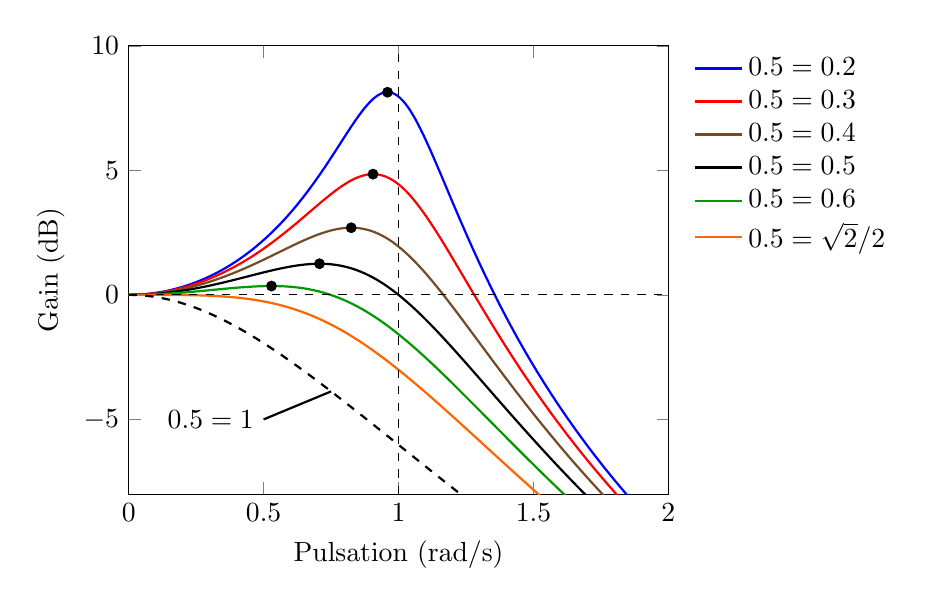
\begin{tikzpicture}
        \pgfplotscreateplotcyclelist{mycolorlist}{%
            blue\\%
            red\\%
            brown!60!black\\%
            black\\%
            green!60!black\\%
            red!60!yellow\\
            }
        \begin{axis}[
            ticklabel style = {font=\normalsize},
            legend style={draw=none},
            legend pos=outer north east,        
            legend cell align={left},
            ylabel={Gain (dB)},
            xlabel={Pulsation (rad/s)},
            xmode=normal,ymode=normal,
            xmin=0.0, xmax=2,
            ymin=-8, ymax=10,
            %grid=both,
            major grid style={black!40},
            cycle list name=mycolorlist,
        ]
        \foreach \a in {0.2,0.3,0.4,0.5,0.6,0.707}
            \addplot+[thick,domain=0:2, samples=501] {-20*log10(sqrt((1-x*x)^2 +(2*\a*x)^2 ))}; 
        \addplot[dashed,domain=0.1:5, samples=201] {0};
        \def\a{1.0}
        \addplot [dashed,thick,domain=0:2, samples=501] {-20*log10(sqrt((1-x*x)^2 +(2*\a*x)^2 ))}; 
        \coordinate (P) at (axis cs:0.75,{-20*log10(sqrt((1-0.75*0.75)^2 +(2*\a*0.75)^2 ))});
        \node[left] (a) at (axis cs:0.5,-5) {$\xi=1$};
        \draw [thick] (a.east) -- (P);
                \addplot[mark size=1.75pt,color = black,fill=black,mark=*,only marks] coordinates {
        	(0.959166304663,8.13608784305)
        	(0.905538513814,4.84656106912)
        	(0.824621125124,2.69540739954)
        	(0.707106781187,1.24938736608)
        	(0.529150262213,0.354575339209)
       	};
        \draw[dashed] (axis cs:1,-10) -- (axis cs:1,10);
            \legend{$\xi=0.2$,$\xi=0.3$,$\xi=0.4$,$\xi=0.5$,$\xi=0.6$,$\xi=\sqrt{2}/2$}
        \end{axis}
    \end{tikzpicture}
    \caption{\'Evolution du gain en décibel en fonction de la pulsation pour différentes
    valeurs du taux d'amortissement du régime pseudo-périodique. Le gain maximal à la pulsation 
    de résonance $\omega_r$ est représenté par une pastille noir sur chacune des courbes pour $\xi<\sqrt{2}/2$.
    On remarquera l'utilisation exceptionnel d'une échelle linéaire pour les pulsations.\label{fig-gain_2nd}}
\end{figure}
\afterpage{\clearpage}
\newpage

%%%%%%%%%%%%%%%%%%%%%%%%%%%%%%%%%%%%%%%%%%%%%%%%%%%%%%%%%%%%%%%%%%%%%%%%%%%%%%%%%%%%%%%%%%%%%%%%%%%%%%%%%%%%
\subsubsection{Diagramme de Bode d'un système d'ordre quelconque}
%%%%%%%%%%%%%%%%%%%%%%%%%%%%%%%%%%%%%%%%%%%%%%%%%%%%%%%%%%%%%%%%%%%%%%%%%%%%%%%%%%%%%%%%%%%%%%%%%%%%%%%%%%%%
Dans le cas d'un système d'ordre supérieur à deux, nous allons utiliser les propriétés d'additivité des diagrammes 
de Bode, en décomposant la fonction de transfert en différents modèles simples.

Il est notamment toujours possible d'écrire une fonction de transfert sous la forme d'un produit gain pur, d'intégrateur, de 
dérivateur, de premier et second ordre: 
\begin{bequation}[ams align]
H(p)= K_0p^{\alpha}\prod_{i} (1+\tau_ip)^{n_i}\prod_{j} (1+2\xi_j\tau_jp+\tau_jp^2)^{n_j}
\end{bequation}
où les exposants $\alpha$, $n_i$ et $n_j$ peuvent être positifs et négatifs. 

Nous listons ci-dessous l'effet sur le gain et la phase d'un diagramme de Bode 
pour chacuns de ces élements selon le signe des exposants $\alpha$, $n_i$, et $n_j$.

\begin{itemize}
    \item le terme $K_0$ (i.e gain pur) provoque:
        \begin{itemize}
            \item gain  : $+20\log{K_0}$
            \item phase : rien 
        \end{itemize}
    \item le terme $K_0p^{\alpha}$ (i.e intégrateur si $\alpha<0$ ou dérivateur si $\alpha>0$)
        provoque :
        \begin{itemize}
            \item gain  : pente de 20$\alpha$ dB/décade 
            \item phase : 90$\alpha$\degree
        \end{itemize}
    \item un terme $\dfrac{1}{(1+\tau_ip)}$ (i.e premier ordre au dénominateur) provoque, en $\omega=\frac{1}{\tau_i}$
        \begin{itemize}
            \item gain  : une rupture de pente de -20 dB/décade 
            \item phase : un saut de -90\degree
        \end{itemize}
    \item un terme $(1+\tau_ip)$ (i.e premier ordre au numérateur) provoque, en $\omega=\frac{1}{\tau_i}$
        \begin{itemize}
            \item gain  : une rupture de pente de +20 dB/décade 
            \item phase : un saut de +90\degree
        \end{itemize}
    \item un terme $\dfrac{1}{(1+2\xi_j\tau_jp+\tau_jp^2)}$ (i.e second ordre au dénominateur) provoque, en $\omega=\frac{1}{\tau_j}$
        \begin{itemize}
            \item gain  : une rupture de pente de -40 dB/décade 
            \item phase : un saut de -180\degree
        \end{itemize}
    \item un terme $(1+2\xi_j\tau_jp+\tau_jp^2)$ (i.e second ordre au numérateur) provoque, en $\omega=\frac{1}{\tau_j}$
        \begin{itemize}
            \item gain  : une rupture de pente de +40 dB/décade 
            \item phase : un saut de +180\degree
        \end{itemize}
\end{itemize}

%%%%%%%%%%%%%%%%%%%%%%%%%%%%%%%%%%%%%%%%%%%%%%%%%%%%%%%%%%%%%%%%%%%%%%%%%%%%%%%%%%%%%%%%%%%%%%%%%%%%%%%%%%%%
\subsection*{Exemple}
%%%%%%%%%%%%%%%%%%%%%%%%%%%%%%%%%%%%%%%%%%%%%%%%%%%%%%%%%%%%%%%%%%%%%%%%%%%%%%%%%%%%%%%%%%%%%%%%%%%%%%%%%%%%

Soit la fonction de transfert $H(p)$ telle que 

\begin{align}
    H(p) = \dfrac{100(p+1)^2}{(100p+1)(10p+1)(0.01p+1)}\label{eq-ft_qq}
\end{align}
La première étape consiste à ordonner les temps caractéristiques par ordre décroissant 
(ou encore les pulsations propres par ordre croissant). Ensuite, il faut identifier 
les différents modèles, ici nous identifions :
\begin{itemize}
    \item un gain pur $K_0=100$
    \item un second ordre double au numérateur de temps caractéristique $\tau=1$
    \item trois premier ordre au dénominateur de temps caractéristique $\tau=\{0.01,10,100\}$
\end{itemize}

Enfin, nous regroupons dans un tableau l'effet 
sur le gain et la phase pour chaque domaines en pulsations compris entre les 
différentes pulsations caractéristiques.
On adopte la notation suivante : $\tau_1=100$, $\tau_2=10$, $\tau_3=1$ et $\tau_4=0.01$, avec $\omega_i=1/\tau_i$, 
on obtient alors:
$\omega_1=0.01$, $\omega_2=0.1$, $\omega_3=1$ et $\omega_4=100$

\begin{table}[!h]
    \resizebox{\linewidth}{!}{
    \begin{tabular}{M{1cm}M{2.5cm}M{2.5cm}M{2.5cm}M{2.5cm}M{2.5cm}N}
    \hhline{======}
    & $\omega\ll\omega_1$ 
    & $\omega_1<\omega<\omega_2$ 
    & $\omega_2<\omega<\omega_3$  
    & $\omega_3<\omega<\omega_4$ 
    & $\omega\gg\omega_4$ & \\[1em]
    \hhline{======}
    $G_{dB}(\omega)$ (pente) & 0(40dB)    &-20dB/décade &-20dB/décade & +40dB/décade & -20dB/décade &\\[1em]
    \hline
    $\phi(\omega)$           & 0\degree   &-90\degree   & -90\degree  & +180\degree  & -90\degree   &\\[1em]
    \hhline{======}
    $G_{dB}(\omega)$ total   & 0(40dB)    &-20dB/décade & -40dB/décade& 0(-20dB)     & -20dB/décade &\\[1em]
    \hline
    $\phi(\omega)$   total   & 0\degree   &-90\degree   &-180\degree  & 0            & -90\degree   &\\[1em]
    \hhline{======}
    \end{tabular}
}
\end{table}


\begin{figure}[!t]
\centering
\begin{tikzpicture}[trim axis left]
\begin{axis}[
    ticklabel style = {font=\footnotesize},
    width=0.9\textwidth,
    height=0.25\textheight,
    ylabel={Gain (dB)},
    xtick={1e-4,1e-3,1e-2,1e-1,1,1e1,1e2,1e3,1e4,1e5}, 
    ytick={-80,-60,-40,-20,0,20,40,60}, 
    xticklabels={$10^{-4}$,$10^{-3}$,$10^{-2}$,$10^{-1}$,$10^{0}$,$10^{1}$,$10^{2}$,$10^{3}$,$10^{4}$,$10^{5}$},
    yticklabels={-80,-60,-40,-20,0,20,40,60}, 
    xmode=log,ymode=normal,
    xmin=1e-4, xmax=1e5,
    ymin=-80, ymax=60,
    grid=both,
    major grid style={black!40}
]
    \addplot[ultra thick, blue,domain=1e-4:1e5, samples=201] {40+20*log10(1+x*x)-10*log10(1+10000*x*x)-10*log10(1+100*x*x)-10*log10(1+0.0001*x*x)}; 
    \addplot[line width=2pt,red,dashed,domain=1e-4:1e-2, samples=101] {40};
    \addplot[line width=2pt,red,dashed,domain=1e-2:1e-1, samples=101] {-20*log10(x)};
    \addplot[line width=2pt,red,dashed,domain=1e-1:1e0 , samples=101] {-40*log10(x)-20*log10(10)};
    \addplot[line width=2pt,red,dashed,domain=1e0:1e2  , samples=101] {-20};
    \addplot[line width=2pt,red,dashed,domain=1e2:1e5  , samples=101] {-20*log10(x)+20*log10(10)};
\end{axis}
\end{tikzpicture}

\begin{tikzpicture}[trim axis left]
\begin{axis}[
    ticklabel style = {font=\footnotesize},
    width=0.9\textwidth,
    height=0.25\textheight,
    xlabel={Pulsation (rad/s)},
    ylabel={Phase (degré)},
    xtick={1e-4,1e-3,1e-2,1e-1,1,1e1,1e2,1e3,1e4,1e5}, 
    ytick={-180,-135,-90,-45,0}, 
    %ytick={0,45,90,135,180}, 
    %ytick={-90,-45,0}, 
    %yticklabels={-180,-135,-90,-45,0},
    %yticklabels={0,45,90,135,180}, 
    yticklabels={-180,-135,-90,-45,0},
    xticklabels={$10^{-4}$,$10^{-3}$,$10^{-2}$,$10^{-1}$,$10^{0}$,$10^{1}$,$10^{2}$,$10^{3}$,$10^{4}$,$10^{5}$},
    xmode=log,ymode=normal,
    xmin=1e-4, xmax=1e5,
    ymin=-180, ymax=0,
    grid=both,
    major grid style={black!40}
]
    \addplot[ultra thick, blue,domain=1e-4:1e5, samples=201] {2*atan2(x,1)-atan2(100*x,1)-atan2(10*x,1)-atan2(0.01*x,1)}; 
    \addplot[line width=2pt,red,dashed,domain=1e-4:1e-2, samples=101] {0};
    \addplot[line width=2pt,red,dashed,domain=1e-2:1e-1, samples=101] {-90};
    \addplot[line width=2pt,red,dashed,domain=1e-1:1e0 , samples=101] {-180};
    \addplot[line width=2pt,red,dashed,domain=1e0:1e2  , samples=101] {0};
    \addplot[line width=2pt,red,dashed,domain=1e2:1e5  , samples=101] {-90};
    \draw[line width=2pt,red,dashed] (axis cs:0.01,0)  -- (axis cs:0.01,-90);
    \draw[line width=2pt,red,dashed] (axis cs:0.1,-90) -- (axis cs:0.1,-180);
    \draw[line width=2pt,red,dashed] (axis cs:1,-180)  -- (axis cs:1,0);
    \draw[line width=2pt,red,dashed] (axis cs:100,0)   -- (axis cs:100,-90);
\end{axis}
\end{tikzpicture}
    \caption{Diagramme de Bode du système d'ordre quelconque de l'\cref{eq-ft_qq} (bleu) diagramme de Bode réel et (rouge) 
    diagramme de Bode asymptotique.\label{fig-bode_qq}}
\end{figure}

Il est également possible de déterminer la forme analytique du gain et de la phase.
\begin{bequation}[ams align]
    G_{dB}(\omega)=40+20\log{(1+\tau_3^2\omega^2)}-10\log{(1+\tau_1^2\omega^2)(1+\tau_2^2\omega^2)(1+\tau_4^2\omega^2)}
\end{bequation}
et
\begin{bequation}[ams align]
\phi(\omega)=2\arctan{\tau_3\omega}-\arctan{\tau_1\omega}-\arctan{\tau_2\omega}-\arctan{\tau_4\omega} 
\end{bequation}

%%%%%%%%%%%%%%%%%%%%%%%%%%%%%%%%%%%%%%%%%%%%%%%%%%%%%%%%%%%%%%%%%%%%%%%%%ùù
\subsection{Diagrammes de Nyquist: méthodologie générale}
%%%%%%%%%%%%%%%%%%%%%%%%%%%%%%%%%%%%%%%%%%%%%%%%%%%%%%%%%%%%%%%%%%%%%%%%%ùù

Pour chacuns des modèles usuels, nous appliquerons la procédure suivante :
\begin{itemize}                                                                                                               
    \item Définir la fonction de transfert $H(p)$ du modèle pour $p=\jw$                                                      
    \item \'Etablir la partie réelle et imaginaire du nombre complexe $H(\jw)$                                          
    \item Tracer le lieu de Nyquist point par point, pour différentes valeurs de 
        $\omega$ de 0 à $+\infty$, c'est à dire $\Re\left(H(\jw)\right)$ 
          et $\Im\left(H(\jw)\right)$ dans le plan complexe.
\end{itemize}
Dans chacuns des exemples suivants nous reproduisons le lieu de Nyquist complet le domaine des pulsations
négatives étant représenté en pointillé. Dans la pratique, il suffit de tracer le symétrique par rapport à 
l'axe des réels et d'inverser le sens de la flêche pour obtenir le sens de la pulsation de $-\infty\to 0$. 
\newpage
%%%%%%%%%%%%%%%%%%%%%%%%%%%%%%%%%%%%%%%%%%%%%%%%%%%%%%%%%%%%%%%%%%%%%%%%%ùù
\subsubsection{Diagramme de Nyquist d'un gain pur}
%%%%%%%%%%%%%%%%%%%%%%%%%%%%%%%%%%%%%%%%%%%%%%%%%%%%%%%%%%%%%%%%%%%%%%%%%ùù
Le diagramme de Nyquist d'un gain pur est trivial. En effet le nombre complexe $H(\jw)$ étant égal 
à une constante réel $K$, le diagramme de Nyquist ce limite à un point sur l'axe des réels quelque soit la valeur de $\omega$.
Ce qui est en accord avec le fait qu'un gain pur présente un déphasage nul.
\begin{align*}
    \Re\left(H(\jw)\right)&=K\\
    \Im\left(H(\jw)\right)&=0\\
\end{align*}

\begin{figure}[!h]                                                                                                           
\begin{center}                                                                                                               
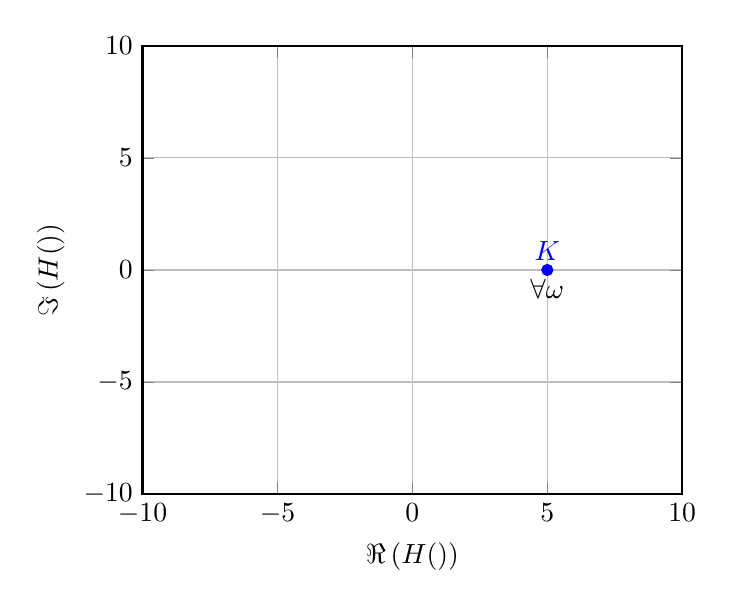
\begin{tikzpicture}
\begin{axis}
    [
    axis line style = thick,
    xlabel=$\Re\left(H(\jw)\right)$,
    ylabel=$\Im\left(H(\jw)\right)$,
    ymin=-10,
    ymax=+10,
    xmin=-10,
    xmax=+10,
    grid=both,
    ]     
    \node [below]       at (axis cs:  5, 0)   {$\forall\omega$};                
    \node [above,blue]       at (axis cs:  5, 0)   {$K$};                
    \addplot [blue, mark = *] coordinates {(5, 0)} {};                          
\end{axis}
\end{tikzpicture}
\end{center}
\caption{Diagramme de Nyquist d'un gain pur. Le nombre complexe 
    $H(\jw)$ est représenté par un point sur l'axe des réels à la valeur $K$ (ici $K=5$).\label{fig-nyquist_1}}
\end{figure}


\newpage
%%%%%%%%%%%%%%%%%%%%%%%%%%%%%%%%%%%%%%%%%%%%%%%%%%%%%%%%%%%%%%%%%%%%%%%%%ùù
\subsubsection{Diagramme de Nyquist d'un intégrateur pur}
%%%%%%%%%%%%%%%%%%%%%%%%%%%%%%%%%%%%%%%%%%%%%%%%%%%%%%%%%%%%%%%%%%%%%%%%%ùù
Le diagramme de Nyquist d'un intégrateur pur est également trivial, puisque 
le nombre complexe $H(\jw)=\dfrac{K}{\jw}$ est un nombre imaginaire pur. 
Cependant il dépend de la pulsation $\omega$.
\begin{align*}
    \Re\left(H(\jw)\right)&=0\\
    \Im\left(H(\jw)\right)&=\dfrac{-K}{\omega}
\end{align*}
\begin{figure}[!h]
\begin{center}
\begin{tikzpicture}
\begin{axis}
    [
    axis line style = thick,
    xlabel=$\Re\left(H(\jw)\right)$,
    ylabel=$\Im\left(H(\jw)\right)$,
    ymin=-10,
    ymax=+10,
    xmin=-10,
    xmax=+10,
    grid=both,
    ] 
    \node [above right] at (axis cs:  0, -10)       {$\omega=0^+$};
    \node [below right] at (axis cs:  0,  10)       {$\omega=0^-$};
    \node [below right]       at (axis cs:  0, 0)   {$\omega\rightarrow+\infty$};
    \node [above right]       at (axis cs:  0, 0)   {$\omega\rightarrow-\infty$};
    \addplot [blue, mark = *] coordinates {(0, 0)} {};
    \addplot[blue,thick,domain=0.01:0.2,samples=50,-{Latex[length=3mm]},unbounded coords=jump] (0,{-1/x});
    \addplot[blue,thick,domain=0.1:100,samples=50,unbounded coords=jump] (0,{-1/x});
    \addplot [dashed,blue,thick,domain=-100:-0.2,-{Latex[length=3mm]},samples=100,unbounded coords=jump](0,{-1/x});
    \addplot [dashed,blue,thick,domain=-0.2:-0.01,samples=100,unbounded coords=jump](0,{-1/x});
\end{axis}
\end{tikzpicture}
\end{center}
\caption{Diagramme de Nyquist d'un intégrateur pur. Le lieu de Nyquist 
    est représenté par une demi droite sur l'axe des nombres 
    imaginaires purs négatifs.\label{fig-nyquist_2}}
\end{figure}

\newpage
%%%%%%%%%%%%%%%%%%%%%%%%%%%%%%%%%%%%%%%%%%%%%%%%%%%%%%%%%%%%%%%%%%%%%%%%%ùù
\subsubsection{Diagramme de Nyquist d'un dérivateur pur}
%%%%%%%%%%%%%%%%%%%%%%%%%%%%%%%%%%%%%%%%%%%%%%%%%%%%%%%%%%%%%%%%%%%%%%%%%ùù
Le diagramme de Nyquist d'un dérivateur pur est également représentatif d'un 
nombre complexe $H(\jw)=K\jw$ imaginaire pur. 
\begin{align*}
    \Re\left(H(\jw)\right)&=0\\
    \Im\left(H(\jw)\right)&=K\omega
\end{align*}
\begin{figure}[!h]                                                                                                           
\begin{center}                                                                                                               
\begin{tikzpicture}
\begin{axis}
    [
    %height=5cm,
    %width=5cm,
    %axis lines = center,
    %ticks=none,
    axis line style = thick,
    %enlargelimits=false,
    xlabel=$\Re\left(H(\jw)\right)$,
    ylabel=$\Im\left(H(\jw)\right)$,
    %xlabel style={below right},
    %ylabel style={left},
    ymin=-10,
    ymax=+10,
    xmin=-10,
    xmax=+10,
    grid=both,
%    clip=false,
    ]     
    \node [below right] at (axis cs:  0, 10)  {$\omega\rightarrow\infty$};                
    \node [above right] at (axis cs:  0,-10)  {$\omega\rightarrow-\infty$};                
    \node [below right]       at (axis cs:  0, 0)   {$\omega=0$};                
    \addplot [blue, mark = *] coordinates {(0, 0)} {};                          
    \addplot [blue,thick,domain=0:5,samples=50,-{Latex[length=3mm]}](0,{x}); 
    \addplot [blue,thick,domain=4:10,samples=50](0,{x}); 
    \addplot [dashed,blue,thick,domain=-10:-5,samples=50,-{Latex[length=3mm]}](0,{x}); 
    \addplot [dashed,blue,thick,domain=-6:0,samples=50](0,{x}); 
\end{axis}
\end{tikzpicture}
\end{center}
\caption{Diagramme de Nyquist d'un dérivateur pur. Le lieu de Nyquist 
    est représenté par une demi droite sur l'axe des nombres 
    imaginaires purs positifs.\label{fig-nyquist_3}}
\end{figure}

\newpage
%%%%%%%%%%%%%%%%%%%%%%%%%%%%%%%%%%%%%%%%%%%%%%%%%%%%%%%%%%%%%%%%%%%%%%%%%ùù
\subsubsection{Diagramme de Nyquist d'un retard pur}
%%%%%%%%%%%%%%%%%%%%%%%%%%%%%%%%%%%%%%%%%%%%%%%%%%%%%%%%%%%%%%%%%%%%%%%%%ùù
\index{Retard pur ! Diagramme de Nyquist}
La fonction de transfert d'un retard pur s'écrit :
$$
H(\jw)=e^{-j\tau\omega}
$$

\begin{figure}[!h]                                                                                                           
\begin{center}                                                                                                               
\begin{tikzpicture}
\begin{axis}
    [
    %height=5cm,
    %width=5cm,
    %axis lines = center,
    %ticks=none,
    axis line style = thick,
    %enlargelimits=false,
    xlabel=$\Re\left(H(\jw)\right)$,
    ylabel=$\Im\left(H(\jw)\right)$,
    %xlabel style={below right},
    %ylabel style={left},
    ymin=-1.5,
    ymax=+1.5,
    xmin=-1.5,
    xmax=+1.5,
    grid=both,
%    clip=false,
    ]     
%    \node [below right] at (axis cs:  0, 10)  {$\omega\rightarrow\infty$};                
%    \node [above right] at (axis cs:  0,-10)  {$\omega\rightarrow-\infty$};                
    \node [right]       at (axis cs:  1, 0)   {\scriptsize$\omega=0$};                
    \addplot [blue, mark = *] coordinates {(1, 0)} {};                          
    \addplot [blue,thick,domain=pi/2:-pi/2-0.2,samples=50,-{Latex[length=3mm]}]({cos(deg(x))},{sin(deg(x)}); 
    \addplot [blue,thick,domain=-pi/2:-3*pi/2-0.2,samples=50,-{Latex[length=3mm]}]({cos(deg(x))},{sin(deg(x)}); 
    %    \addplot [dashed,blue,thick,domain=-10:-5,samples=50,-latex]({cos(deg(x))},{sin(deg(x)}); 
    %\addplot [dashed,blue,thick,domain=-6:0,samples=50]({cos(deg(x))},{sin(deg(x)}); 
\end{axis}
\end{tikzpicture}
\end{center}
\caption{Diagramme de Nyquist d'un retard pur. Le lieu de Nyquist 
    est représenté par le cercle unité dans le plan complexe.\label{fig-nyquist_4}}
\end{figure}

\newpage
%%%%%%%%%%%%%%%%%%%%%%%%%%%%%%%%%%%%%%%%%%%%%%%%%%%%%%%%%%%%%%%%%%%%%%%%%ùù
\subsubsection{Diagramme de Nyquist d'un système du premier ordre}
%%%%%%%%%%%%%%%%%%%%%%%%%%%%%%%%%%%%%%%%%%%%%%%%%%%%%%%%%%%%%%%%%%%%%%%%%ùù
\index{Système du 1er ordre ! Diagramme de Nyquist}
La fonction de transfert d'un système du premier ordre s'écrit:
$$
H(\jw)=\dfrac{K}{1+j\tau\omega}
$$
Les parties réelle et imaginaire de cette fonction de transfert sont données par:
\begin{align*}
    \Re\left(H(\jw)\right)&=\dfrac{K}{1+\tau^2\omega^2}\\
    \Im\left(H(\jw)\right)&=-\dfrac{K\tau\omega}{1+\tau^2\omega^2}\\
\end{align*}
Nous avons regroupé dans le~\cref{tab-nyquist-vp_1er} quelques valeurs particulières 
de $\Re\left(H(\jw)\right)$ et $\Im\left(H(\jw)\right)$ pour quelques valeurs de $\omega$.

Le lieu complet de Nyquist d'un système du premier ordre à la forme d'un cercle, nous allons établir
ses caractéristiques\cite{9782729860127}.

Posons tout d'abord,
$$
X=\Re\left(H(\jw)\right)=\dfrac{K}{1+\tau^2\omega^2}
$$
on peut écrire,
$$
\tau^2\omega^2=\dfrac{K}{X}-1
$$
En posant maintenant, 
$$
Y=\Im\left(H(\jw)\right)=\dfrac{\tau\omega}{1+\tau^2\omega}=-\tau\omega X
$$
on obtient une relation entre $Y$ et $X$:
$$
Y^2=\left(\dfrac{K}{X}-1\right)X^2
$$
on reconnait alors l'équation d'un cercle de centre $(K/2,0)$ et de rayon $K/2$
$$
\left(X-\dfrac{K}{2}\right)^2+Y^2=\left(\dfrac{K}{2}\right)^2
$$
\begin{table}
    \begin{center}
    \begin{tabular}{M{2.0cm}M{2.0cm}M{2.0cm}M{2.0cm}N}
        \hhline{====}
                                     & $\omega=0$  & $\omega\to\infty$    & $\omega=\dfrac{1}{\tau}$ & \\[1.5em]
        \hline
        $\Re\left(H(\jw)\right)$     & $K$         & 0                    & $K/2$                    & \\ [1.5em]
        \hline
        $\Im\left(H(\jw)\right)$     & 0           & 0                    & $-K/2$                     & \\[1.5em]
        \hhline{====}
    \end{tabular}
    \caption{Quelques valeurs particulières de $\Re\left(H(\jw)\right)$ et $\Im\left(H(\jw)\right)$
    selon $\omega$ pour un système du premier ordre\label{tab-nyquist-vp_1er}.}
    \end{center}
\end{table}

\begin{figure}[!h]                                                                                                           
\begin{center}                                                                                                               
\begin{tikzpicture}                                                                 
\begin{axis}                                                                        
    [                                                                               
    %height=5cm,                                                                     
    %width=5cm,                                                                      
    axis line style = thick,                                                        
%    enlargelimits=false,                                                            
    xlabel=$\Re\left(H(\jw)\right)$,                                                
    ylabel=$\Im\left(H(\jw)\right)$,                                                
%    xlabel style={below right},                                                     
%    ylabel style={left},                                                            
    ymin=-0.75,                                                                       
    ymax=+0.75,                                                                       
    xmin=-0.3,                                                                       
    xmax=+1.3,                                                                       
    clip=false,                                                                     
    grid=both
    ]                                                                               
    \addplot [blue,thick,domain=0:1.1,samples=100,-{Latex[length=3mm]}]({1/(1+x*x)},{-x/(1+x*x)}); 
    \addplot [blue,thick,domain=0.5:5,samples=100]({1/(1+x*x)},{-x/(1+x*x)}); 
    \addplot [blue,thick,domain=5:10,samples=100]({1/(1+x*x)},{-x/(1+x*x)}); 
    \addplot [blue,thick,domain=10:100,samples=100]({1/(1+x*x)},{-x/(1+x*x)}); 

    \addplot [dashed,blue,thick,domain=-100:-10,samples=100]({1/(1+x*x)},{-x/(1+x*x)}); 
    \addplot [dashed,blue,thick,domain=-10:-5,samples=100]({1/(1+x*x)},{-x/(1+x*x)}); 
    \addplot [dashed,blue,thick,domain=-5:-0.5,samples=100,-{Latex[length=3mm]}]({1/(1+x*x)},{-x/(1+x*x)}); 
    \addplot [dashed,blue,thick,domain=-0.5:0,samples=100]({1/(1+x*x)},{-x/(1+x*x)}); 

    \node [above left,xshift=0.2em] at (axis cs:  0, 0)  {\scriptsize$\omega\rightarrow-\infty$};         
    \node [below left,xshift=0.2em] at (axis cs:  0, 0)  {\scriptsize$\omega\rightarrow+\infty$};         
    \node [right]       at (axis cs:  1, 0) {\scriptsize$\omega=0$};                        
    \addplot [blue, mark = *] coordinates {(0, 0)} {};                             
    \addplot [blue, mark = *] coordinates {(1, 0)} {};                             
%    \draw[blue,ultra thick,-latex] (axis cs:  0,  0 ) -- (axis cs:  0, 5 );        
%    \draw[blue,ultra thick] (axis cs:  0,  4 ) -- (axis cs:  0, 9 );               
\end{axis}                                                                          
\end{tikzpicture}                                                                   
\end{center}
\caption{Diagramme de Nyquist d'un système du premier ordre. 
    Avec $K=1$ et $\tau=1$. Le lieu de Nyquist 
    est représenté par un demi cercle idans le plan des nombres 
    imaginaires négatifs. Le lieu de Nyquist complet correspond à un cercle de rayon $K/2$ et de centre $(K/2,0)$ 
    \label{fig-nyquist_1er}}
\end{figure}


\newpage
%%%%%%%%%%%%%%%%%%%%%%%%%%%%%%%%%%%%%%%%%%%%%%%%%%%%%%%%%%%%%%%%%%%%%%%%%ùù
\subsubsection{Diagramme de Nyquist d'un système du second ordre}
%%%%%%%%%%%%%%%%%%%%%%%%%%%%%%%%%%%%%%%%%%%%%%%%%%%%%%%%%%%%%%%%%%%%%%%%%ùù
\index{Système du second ordre ! Diagramme de Nyquist}
La fonction de transfert d'un système du second ordre s'écrit:
$$
H(\jw)=\dfrac{K\omega_0^2}{(\omega_0^2-\omega^2)+j2\xi\omega_0\omega}
$$
Les parties réel et imaginaire de cette fonction de transfert sont données par:
\begin{align*}
    \Re\left(H(\jw)\right)&=\dfrac{K\omega_0^2(\omega_0^2-\omega^2)}{(\omega_0^2-\omega^2)^2+4\xi^2\omega_0^2\omega^2}\\
    \Im\left(H(\jw)\right)&=\dfrac{-2\xi\omega_0^2\omega^2}{(\omega_0^2-\omega^2)^2+4\xi^2\omega_0^2\omega^2}\\
\end{align*}
\begin{figure}[!h]                                                                                                           
\begin{center}                                                                                                               
\begin{tikzpicture}                                                                 
\begin{axis}                                                                        
    [                                                                               
    axis line style = thick,                                                        
    xlabel=$\Re\left(H(\jw)\right)$,                                                
    ylabel=$\Im\left(H(\jw)\right)$,                                                
    ymin=-1.5,                                                                       
    ymax=+1.5,                                                                       
    xmin=-0.5,                                                                       
    xmax=+1.3,                                                                       
    clip=false,                                                                     
    grid=both
    ]                                                                               
    \tikzstyle{lieua}=[blue,thick,samples=150,-{Latex[length=3mm]}]
    \tikzstyle{lieu}=[blue,thick,samples=150]
    \tikzstyle{lieua_c}=[dashed,blue,thick,samples=150,-{Latex[length=3mm]}]
    \tikzstyle{lieu_c}=[dashed,blue,thick,samples=150]
    
    \def\xi{0.5}
    \addplot[lieua,domain=0:1]({(1-x^2)/((1-x^2)^2+4*\xi^2*x^2)},{-(2*\xi*x)/((1-x^2)^2+4*\xi^2*x^2)}); 
    \addplot[lieu, domain=0.99:5]({(1-x^2)/((1-x^2)^2+4*\xi^2*x^2)},{-(2*\xi*x)/((1-x^2)^2+4*\xi^2*x^2)}); 
    \addplot[lieu,domain=5:10]({(1-x^2)/((1-x^2)^2+4*\xi^2*x^2)},{-(2*\xi*x)/((1-x^2)^2+4*\xi^2*x^2)}); 
    \addplot[lieu,domain=10:100]({(1-x^2)/((1-x^2)^2+4*\xi^2*x^2)},{-(2*\xi*x)/((1-x^2)^2+4*\xi^2*x^2)}); 

    \addplot[lieu_c,domain=-100:-10]({(1-x^2)/((1-x^2)^2+4*\xi^2*x^2)},{-(2*\xi*x)/((1-x^2)^2+4*\xi^2*x^2)}); 
    \addplot[lieu_c,domain=-10:-5]({(1-x^2)/((1-x^2)^2+4*\xi^2*x^2)},{-(2*\xi*x)/((1-x^2)^2+4*\xi^2*x^2)}); 
    \addplot[lieua_c,domain=-5:-0.99]({(1-x^2)/((1-x^2)^2+4*\xi^2*x^2)},{-(2*\xi*x)/((1-x^2)^2+4*\xi^2*x^2)}); 
    \addplot[lieu_c,domain=-0.99:0]({(1-x^2)/((1-x^2)^2+4*\xi^2*x^2)},{-(2*\xi*x)/((1-x^2)^2+4*\xi^2*x^2)});

    \node [above right] at (axis cs:  0, 0)  {\scriptsize$\omega\rightarrow-\infty$};
    \node [right]       at (axis cs:  1, 0)  {\scriptsize$\omega=0$};       
    \node [below right] at (axis cs:  0, 0)  {\scriptsize$\omega\rightarrow+\infty$};
    \addplot [blue, mark = *] coordinates {(0, 0)} {};                  
    \addplot [blue, mark = *] coordinates {(1, 0)} {};                  
\end{axis}                                                                          
\end{tikzpicture}                                                                   
\end{center}
\caption{Diagramme de Nyquist d'un système du second ordre. 
    Avec $K=1$ et $\tau=1$. Le lieu de Nyquist est représenté par une demi cardio\"iode dans le plan
    des nombres imaginaires négatifs.\label{fig-nyquist_2nd_1}}
\end{figure}

\begin{figure}[!h]                                                                                                           
\begin{center}                                                                                                               
\begin{tikzpicture}                                                                 
        \pgfplotscreateplotcyclelist{mycolorlist}{%
            blue\\%
            blue\\%
            blue\\%
            blue\\%
            blue\\%
            blue\\%
            blue\\%
            blue\\%
            red\\%
            red\\%
            red\\%
            red\\%
            red\\%
            red\\%
            red\\%
            red\\%
            brown!60!black\\%
            brown!60!black\\%
            brown!60!black\\%
            brown!60!black\\%
            brown!60!black\\%
            brown!60!black\\%
            brown!60!black\\%
            brown!60!black\\%
            black\\%
            black\\%
            black\\%
            black\\%
            black\\%
            black\\%
            black\\%
            black\\%
            }
\begin{axis}                                                                        
    [                                                                               
    name=nyq1,
    axis line style = thick,
    xlabel=$\Re\left(H(\jw)\right)$,
    ylabel=$\Im\left(H(\jw)\right)$,
    ymin=-2,
    ymax=+2,
    xmin=-0.8,
    xmax=+1.3,
    grid=both,
    cycle list name=mycolorlist,
    legend style={draw=none,yshift=1em},    
    legend pos=outer north east, 
    ]                                                                               
    \tikzstyle{lieua}=[thick,samples=100,-{Latex[length=3mm]}]
    \tikzstyle{lieu}=[thick,samples=100]
    \tikzstyle{lieua_c}=[dashed,thick,samples=100,-{Latex[length=3mm]}]
    \tikzstyle{lieu_c}=[dashed,thick,samples=100]
                                                                                                                             
    \foreach \xi in {0.4,0.6,0.8,1.0} 
    {
    \addplot+[lieua,domain=0:1]       ({(1-x^2)/((1-x^2)^2+4*\xi^2*x^2)},{-(2*\xi*x)/((1-x^2)^2+4*\xi^2*x^2)});
    \addplot+[lieu, domain=0.99:5]    ({(1-x^2)/((1-x^2)^2+4*\xi^2*x^2)},{-(2*\xi*x)/((1-x^2)^2+4*\xi^2*x^2)});
    \addplot+[lieu,domain=5:10]       ({(1-x^2)/((1-x^2)^2+4*\xi^2*x^2)},{-(2*\xi*x)/((1-x^2)^2+4*\xi^2*x^2)});
    \addplot+[lieu,domain=10:100]     ({(1-x^2)/((1-x^2)^2+4*\xi^2*x^2)},{-(2*\xi*x)/((1-x^2)^2+4*\xi^2*x^2)});
                                                                                                                              
    \addplot+[lieu_c,domain=-100:-10] ({(1-x^2)/((1-x^2)^2+4*\xi^2*x^2)},{-(2*\xi*x)/((1-x^2)^2+4*\xi^2*x^2)});
    \addplot+[lieu_c,domain=-10:-5]   ({(1-x^2)/((1-x^2)^2+4*\xi^2*x^2)},{-(2*\xi*x)/((1-x^2)^2+4*\xi^2*x^2)});
    \addplot+[lieua_c,domain=-5:-0.99]({(1-x^2)/((1-x^2)^2+4*\xi^2*x^2)},{-(2*\xi*x)/((1-x^2)^2+4*\xi^2*x^2)});
    \addplot+[lieu_c,domain=-0.99:0]  ({(1-x^2)/((1-x^2)^2+4*\xi^2*x^2)},{-(2*\xi*x)/((1-x^2)^2+4*\xi^2*x^2)});
    }
    \legend{,$\xi=0.4$,,,,,,,,$\xi=0.6$,,,,,,,,$\xi=0.8$,,,,,,,,$\xi=1.0$,,,,,,,} 
\end{axis}                                                                          
        \pgfplotscreateplotcyclelist{mycolorlist}{%
            blue\\%
            blue\\%
            blue\\%
            blue\\%
            blue\\%
            blue\\%
            red\\%
            red\\%
            red\\%
            red\\%
            red\\%
            red\\%
            brown!60!black\\%
            brown!60!black\\%
            brown!60!black\\%
            brown!60!black\\%
            brown!60!black\\%
            brown!60!black\\%
            black\\%
            black\\%
            black\\%
            black\\%
            black\\%
            black\\%
            }
\begin{axis}                                                                        
    [                                                                               
    at={(nyq1.below south west)},yshift=-0.2cm,anchor=north west,
    axis line style = thick,
    xlabel=$\Re\left(H(\jw)\right)$,
    ylabel=$\Im\left(H(\jw)\right)$,
    ymin=-15,
    ymax=+15,
    xmin=-6,
    xmax=+6,
    grid=both,
    cycle list name=mycolorlist,
    legend style={draw=none,yshift=1em},    
    legend pos=outer north east, 
    ]
    \tikzstyle{lieua}=[thick,samples=200,-{Latex[length=3mm]}]
    \tikzstyle{lieu}=[thick,samples=200]
    \tikzstyle{lieua_c}=[dashed,thick,samples=200,-{Latex[length=3mm]}]
    \tikzstyle{lieu_c}=[dashed,thick,samples=200]
                                                                                                                             
    \foreach \xi in {0.05,0.07,0.1,0.2} 
%    \foreach \xi in {0.05} 
    {
    \addplot+[lieu,domain=0:0.5]      ({(1-x^2)/((1-x^2)^2+4*\xi^2*x^2)},{-(2*\xi*x)/((1-x^2)^2+4*\xi^2*x^2)});
    \addplot+[lieua, domain=0.5:1]    ({(1-x^2)/((1-x^2)^2+4*\xi^2*x^2)},{-(2*\xi*x)/((1-x^2)^2+4*\xi^2*x^2)});
    \addplot+[lieu, domain=0.99:2]    ({(1-x^2)/((1-x^2)^2+4*\xi^2*x^2)},{-(2*\xi*x)/((1-x^2)^2+4*\xi^2*x^2)});
    
    \addplot+[lieua_c,domain=-2:-1.0]   ({(1-x^2)/((1-x^2)^2+4*\xi^2*x^2)},{-(2*\xi*x)/((1-x^2)^2+4*\xi^2*x^2)});
    \addplot+[lieu_c,domain=-1.0:-0.5]  ({(1-x^2)/((1-x^2)^2+4*\xi^2*x^2)},{-(2*\xi*x)/((1-x^2)^2+4*\xi^2*x^2)});
    \addplot+[lieu_c,domain=-0.5:0]   ({(1-x^2)/((1-x^2)^2+4*\xi^2*x^2)},{-(2*\xi*x)/((1-x^2)^2+4*\xi^2*x^2)});
    }
    \legend{$\xi=0.05$,,,,,,$\xi=0.07$,,,,,,$\xi=0.1$,,,,,,$\xi=0.2$,,,,,,} 
\end{axis}                                                                          
\end{tikzpicture}                                                                   
\end{center}
\caption{Diagramme de Nyquist d'un système du second ordre pour différentes valeurs du 
    taux d'amortissement $\xi$. Avec $K=1$ et $\tau=1$. Le lieu de Nyquist est 
    représenté par une demi cardio\"iode dans le plan des imaginaires négatifs.\label{fig-nyquist_2nd_2}}
\end{figure}

\newpage
%%%%%%%%%%%%%%%%%%%%%%%%%%%%%%%%%%%%%%%%%%%%%%%%%%%%%%%%%%%%%%%%%%%%%%%%%%%
\subsubsection{Effet d'un retard sur le diagramme de Nyquist}
%%%%%%%%%%%%%%%%%%%%%%%%%%%%%%%%%%%%%%%%%%%%%%%%%%%%%%%%%%%%%%%%%%%%%%%%%%%
\index{Retard pur ! effet d'un retard sur le diagramme de Nyquist}
La fonction de transfert $H_R(\jw)$ d'un retard est donnée par la relation :
$$
H_R(\jw)=e^{-j\tau_1\omega}=\cos{\tau_1\omega}-j\sin{\tau_1\omega}
$$
avec $\tau_1$ le retard. 
\'Etudions l'effet de ce retard sur le diagramme de Nyquist d'un système du premier ordre $H(\jw)$.
La fonction de transfert modifié est:
$$
H(\jw)=\dfrac{K}{1+j\tau\omega}H_R(\jw)=\dfrac{K}{1+j\tau\omega}\left(\cos{\tau\omega}-j\sin{\tau\omega}\right)
$$
Les parties réels et imaginaire de la fonction de transfert sont:
\begin{align*}
    \Re\left(H(\jw)\right)&=\dfrac{K\left(\cos{\tau_1\omega-\tau\omega\sin{\tau_1\omega}}\right)}{1+\tau^2\omega^2}\\
    \Im\left(H(\jw)\right)&=\dfrac{-K\left(\tau\omega\cos{\tau_1\omega+\sin{\tau_1\omega}}\right)}{1+\tau^2\omega^2}\\
\end{align*}

\begin{figure}[!h]                                                                                                           
\begin{center}                                                                                                               
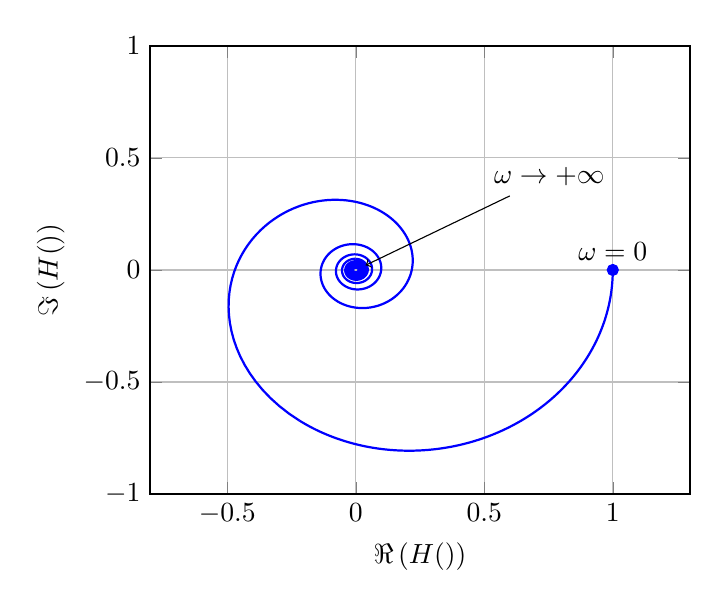
\begin{tikzpicture}                                                                 
\begin{axis}                                                                        
    [                                                                               
    axis line style = thick,                                                        
    xlabel=$\Re\left(H(\jw)\right)$,                                                
    ylabel=$\Im\left(H(\jw)\right)$,                                                
    ymin=-1,                                                                       
    ymax=1,                                                                       
    xmin=-0.8,                                                                       
    xmax=+1.3,                                                                       
    grid=both,
    ]                                                                               
    \def\t{1.0}
    \def\tu{1.1}
    \addplot[blue,thick,domain=0:1,samples=200] 
    ({(cos(deg(\tu*x))-\t*x*sin(deg(\tu*x)))/(1+\t^2*x^2)},{-(\t*x*cos(deg(\tu*x))+sin(deg(\tu*x)))/(1+\t^2*x^2)});
    \addplot[blue,thick,domain=1:10,samples=200] 
    ({(cos(deg(\tu*x))-\t*x*sin(deg(\tu*x)))/(1+\t^2*x^2)},{-(\t*x*cos(deg(\tu*x))+sin(deg(\tu*x)))/(1+\t^2*x^2)});
    \addplot[blue,thick,domain=10:20,samples=200] 
    ({(cos(deg(\tu*x))-\t*x*sin(deg(\tu*x)))/(1+\t^2*x^2)},{-(\t*x*cos(deg(\tu*x))+sin(deg(\tu*x)))/(1+\t^2*x^2)});
    \addplot[blue,thick,domain=20:50,samples=200] 
    ({(cos(deg(\tu*x))-\t*x*sin(deg(\tu*x)))/(1+\t^2*x^2)},{-(\t*x*cos(deg(\tu*x))+sin(deg(\tu*x)))/(1+\t^2*x^2)});
    \addplot[blue,thick,domain=50:100,samples=200] 
    ({(cos(deg(\tu*x))-\t*x*sin(deg(\tu*x)))/(1+\t^2*x^2)},{-(\t*x*cos(deg(\tu*x))+sin(deg(\tu*x)))/(1+\t^2*x^2)});
    \node [above]       at (axis cs:  1, 0)   {$\omega=0$};       
    \addplot [blue, mark = *] coordinates {(1, 0)} {};                             
    \node [below right] (A) at (axis cs:  0.5, 0.5)  {$\omega\rightarrow+\infty$};
    \node (B) at (axis cs:  0, 0)  {};
    \draw[->] (A) -- (B);
\end{axis}                                                                          
\end{tikzpicture}                                                                   
\end{center}
\caption{Effet d'un retard sur le diagramme de Nyquist d'un système du premier ordre. 
    Avec $K=1$, $\tau=1$ et $\tau_1=2$. Le lieu de Nyquist est représenté par 
    une spirale.\label{fig-nyquist}}
\end{figure}

\begin{figure}[!h]                                                                                                           
\begin{center}                                                                                                               
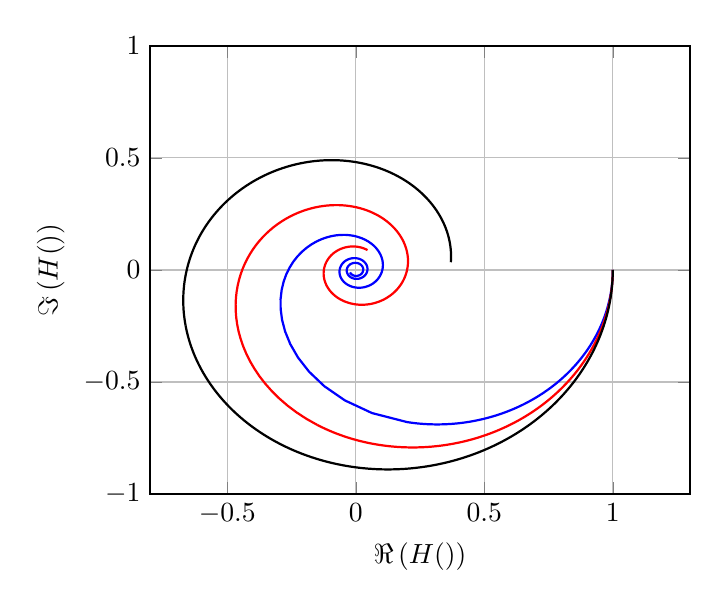
\begin{tikzpicture}                                                                 
        \pgfplotscreateplotcyclelist{mycolorlist}{%
            blue\\%
            blue\\%
            red\\%
            red\\%
            black\\%
            black\\%
            brown!60!black\\%
            brown!60!black\\%
            green!60!black\\%
            green!60!black\\%
            red!60!yellow\\
            red!60!yellow\\
        }
\begin{axis}                                                                        
    [                                                                               
    axis line style = thick,                                                        
    xlabel=$\Re\left(H(\jw)\right)$,                                                
    ylabel=$\Im\left(H(\jw)\right)$,                                                
    ymin=-1,                                                                       
    ymax=1,                                                                       
    xmin=-0.8,                                                                       
    xmax=+1.3,                                                                       
    grid=both,
    cycle list name=mycolorlist,
    ]                                                                               
    \def\t{1.0}
    \def\tu{0.5}

    \foreach \tu in {0.5,1.0,2.0}
    {
    \addplot+[thick,domain=0:1,samples=200] 
    ({(cos(deg(\tu*x))-\t*x*sin(deg(\tu*x)))/(1+\t^2*x^2)},{-(\t*x*cos(deg(\tu*x))+sin(deg(\tu*x)))/(1+\t^2*x^2)});
    \addplot+[thick,domain=1:{10/\tu^2},samples=200] 
    ({(cos(deg(\tu*x))-\t*x*sin(deg(\tu*x)))/(1+\t^2*x^2)},{-(\t*x*cos(deg(\tu*x))+sin(deg(\tu*x)))/(1+\t^2*x^2)});
}
\end{axis}                                                                          
\end{tikzpicture}                                                                   
\end{center}
    \caption{Effet d'un retard sur le diagramme de Nyquist d'un système du premier ordre 
         pour différentes valeurs de retard. (bleu) $\tau_1=0.5$, (rouge) $\tau_1=1.0$ 
         et (noir) $\tau_1=2.0$
         Avec $K=1$, $\tau=1$ et $\tau_1=2$. Le lieu de Nyquist est représenté par 
         une spirale. Par souci de clarté, nous n'avons ici représenté que l'intervalle $\omega\in[0,\dfrac{10}{\tau_1}]$ 
         \label{fig-nyquist}}
\end{figure}

%%%%%%%%%%%%%%%%%%%%%%%%%%%%%%%%%%%%%%%%%%%%%%%%%%%%%%%%%%%%%%%%%%%%%%%%%ùù
\subsection{Diagrammes de Black: méthodologie générale}
%%%%%%%%%%%%%%%%%%%%%%%%%%%%%%%%%%%%%%%%%%%%%%%%%%%%%%%%%%%%%%%%%%%%%%%%%ùù

%%%%%%%%%%%%%%%%%%%%%%%%%%%%%%%%%%%%%%%%%%%%%%%%%%%%%%%%%%%%%%%%%%%%%%%%%ùù
%%%%%%%%%%%%%%%%%%%%%%%%%%%%%%%%%%%%%%%%%%%%%%%%%%%%%%%%%%%%%%%%%%%%%%%%%ùù
\section{Etude du transitoire de la réponse harmonique}
%%%%%%%%%%%%%%%%%%%%%%%%%%%%%%%%%%%%%%%%%%%%%%%%%%%%%%%%%%%%%%%%%%%%%%%%%ùù
%%%%%%%%%%%%%%%%%%%%%%%%%%%%%%%%%%%%%%%%%%%%%%%%%%%%%%%%%%%%%%%%%%%%%%%%%ùù
\acpl
%c.f pdf/[AnaHSLCI][CO]Analyse_harmonique_des_SLCI.pdf
\subsection{Exemple d'un système du premier ordre}
\acpl
\subsection{Exemple d'un système du second ordre}
\acpl

